% $Header:
\pdfminorversion=4 % allow opening in Adobe Reader/Acrobat
\documentclass[10pt]{beamer}
\geometry{paperwidth=170.67mm, paperheight=96mm} % 16:9 aspect ratio

\mode<presentation>
{
  \usetheme{default}
  \usefonttheme{structurebold}
  % or ...
  \setbeamercovered{transparent}
}
% Changes the color of bullets and other fonts to match the NormalANLBlue template
\definecolor{mcmasterred}{RGB}{122 0 60}
\definecolor{mcmastergrey}{RGB}{142 151 157}
\setbeamercolor{structure}{fg=mcmasterred} % for slide titles, etc
\setbeamercolor{block title}{fg=white,bg=mcmasterred} % For blocks
\setbeamercolor{block body}{fg=black,bg=white} % For blocks

\beamertemplatenavigationsymbolsempty

%\usebackgroundtemplate{\includegraphics[width=\paperwidth]{NormalANLBlue}}
\usepackage[dvipsnames]{xcolor}
\usepackage{caption}

\usepackage[english]{babel}
\usepackage[latin1]{inputenc}
\usepackage{times}
\usepackage[T1]{fontenc}
\usepackage{mathshortcuts,bm}
\usepackage{booktabs}          % nicer tables
\usepackage{dcolumn}           % format numeric data in tables
\usepackage{setspace}          % set line spacing
\usepackage{multirow}
\usepackage[version=3]{mhchem} % typeset chemical formula
\usepackage{perpage} % restart footnotes on each page
\MakePerPage{footnote}
\usepackage{nicematrix}

\usepackage{tikz} % flowcharting options
\usetikzlibrary{shapes.geometric, arrows.meta, positioning, patterns}
\definecolor{arrowcolor}{HTML}{262626} % arrow
\definecolor{darkgrey}{HTML}{3A3A3A} % un-selected rectangle 
\definecolor{ZColor}{HTML}{E67E23} 

\newcommand{\makeflowchart}[4]{%
\centerline{
\begin{tikzpicture}[
	block/.style = {
		rectangle, fill=mcmasterred, 
		minimum width=3cm, minimum height = 1cm, text width = 3cm,
		draw=none, text=white, align=center
	},
	altcolor/.style = {fill=arrowcolor},
	arrow/.style = {->, >={stealth[scale=0.50]}, line width=1.5pt, draw=darkgrey}
]

%Set up flowchart
\node[block, fill=#1] (rect1) {Piecewise affine mapping};
\node[block, fill=#2, right=1cm of rect1] (rect2) {Abs-normal form};
\node[block, fill=#3, right=1cm of rect2] (rect3) {Construct LCP coefficients};
\node[block, fill=#4, right=1cm of rect3] (rect4) {Solve LCP};

\draw[arrow] (rect1) -- (rect2);
\draw[arrow] (rect2) -- (rect3);
\draw[arrow] (rect3) -- (rect4);

\end{tikzpicture}}}

%%TITLE PAGE:
\title % (optional, use only with long paper titles)
{New complementarity formulations for \\nonsmooth process models}

\author
{Maha Chaudhry \and Yulan Zhang \and \underline{Kamil A. Khan} \\ \small kamilkhan@mcmaster.ca}
\institute{
  Department of Chemical Engineering, McMaster University
}

\date
{AlChE, Minneapolis\\~\\ Nov 9, 2026}

\subject{Talks}
%%%%

%%OUTLINE:
\AtBeginSection[]
{
  \begin{frame}<beamer>{Outline}
    \tableofcontents[currentsection]
  \end{frame}
}
\setbeamertemplate{footline}[frame number]

%%%%%%%%%%%%%%%%%%%%%%%%%%%%%%%%%%%
\begin{document}
\begin{frame}
  \titlepage
\begin{tikzpicture}[remember picture,overlay]
\node[anchor=north east,yshift=2pt] at (current page.north east) {
\includegraphics[height=1.0cm]{images/mcmasterlogo}};
\end{tikzpicture}
\end{frame}

\usebackgroundtemplate{%
\begin{tikzpicture}[remember picture,overlay]
\node[anchor=north east,yshift=2pt] at (current page.north east) {
\includegraphics[height=0.8cm]{images/mcmasterlogo}};
\end{tikzpicture}}


\section{Motivation and background}

\subsection{Challenges of nonsmoothness}
\begin{frame}[t]
  \frametitle{Challenges of nonsmoothness}
  
  Numerical methods for smooth systems may perform poorly or fail when nonsmoothness is encountered
  \only<1>{
    \begin{block}{Descent directions become difficult to find}
      \begin{itemize}
      \item Negative of a subgradient is not necessarily a descent
        direction
      \item Example: $f(x,y)
        =\max(0.1y+x, \,\, 0.1y-x)$
        %$f:(x,y)\in\reals^2
        %\mapsto\max\{0.1y+x, \,\, 0.1y-x\}$
      	\vspace{-3mm}  
	\begin{figure}
          \centering
          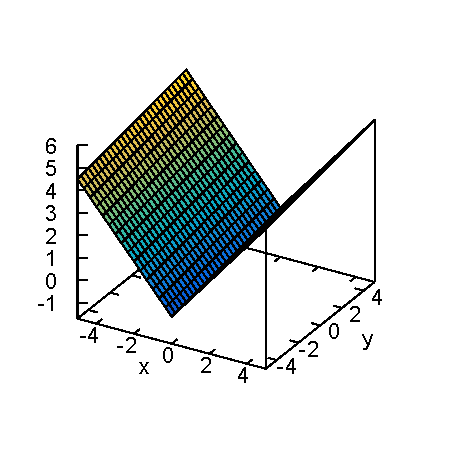
\includegraphics[height=0.6\textheight]{images/figAscent.pdf}
        \end{figure}
      \end{itemize}
    \end{block}
  }

  \only<2>{
    \begin{block}{Reliable methods may fail}
      Example from Hiriart-Urruty and Lemar\'echal (1993):
      \begin{itemize}
      \item $f(x,y) = \max(-100,\,\,3y\pm2x,\,\,2y\pm5x)$
        %$f:(x,y)\in\reals^2
        %\mapsto\max\{-100,\,\,3y\pm2x,\,\,2y\pm5x\}$
	 \vspace{-3mm}
        \begin{figure}
          \centering
          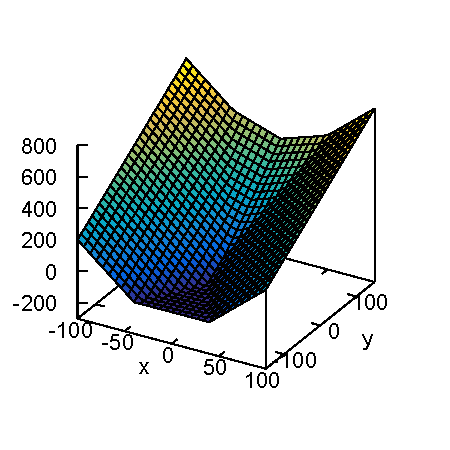
\includegraphics[height=0.6\textheight]{images/figSteep.pdf}
        \end{figure}
	\vspace{-5mm}
      \item Failure of steepest descent with exact line search
      \end{itemize}
    \end{block}
  }
\end{frame}

\begin{frame}{Nonsmoothness in applications}
\begin{itemize}\setlength{\itemsep}{10pt}
  \item Modeling discrete-continuous phenomena
  \begin{itemize}
      \item thermodynamic phase changes
      \item multi-stage processes (e.g. pressure-swing adsorption)
  \end{itemize}
  \item Activation of safety mechanisms
    \begin{itemize}
    \item check valves, relief valves
    \end{itemize}
  \item Embedded optimization problems
    \begin{itemize}
    \item dynamic flux balance analysis (Hjersted and Henson, 2009)
    \item closed-form optimal control
    \end{itemize}
  \item Aggressive penalty methods for constrained optimization
  \item Neural networks (e.g., ReLU activation)
  \end{itemize}
\end{frame}

\subsection{Neural Networks}
\begin{frame}{Neural Network Architecture}
	%\begin{block}{Neural Network Architecture}
	%\vspace{2mm}
		\begin{minipage}{0.54\textwidth}
			From Aydinoglu et al. [2021], a NN $\pmb{\phi}(\mathbf{x})$ is a \\multilayer perceptron with $L$ hidden layers:
			\begin{equation*}
				\pmb{\phi}(\mathbf{x}) = (\mathbf{h}^{(L+1)} \circ \pmb{\lambda}_{ReLU} \circ \mathbf{h}^{(L)} \circ ... \pmb{\lambda}_{ReLU} \circ \mathbf{h}^{(1)})(\mathbf{x})
			\end{equation*}
			\vspace{-5.5mm}
			\begin{itemize}
				\item \textbf{Affine function} ($\mathbf{h}^{(\ell)}$) - describing weighted linear relationship between neurons between hidden layers. It satisfies: \(\mathbf{h}^{(\ell)}(\mathbf{x}) = \pmb{\theta}^{(\ell)}\mathbf{x} + \mathbf{C}^{(\ell)}\) 
				\vspace{2mm}
				\item \textbf{Activation function} ($\pmb{\lambda}_{ReLU}$) satisfies \(\pmb{\lambda}_{ReLU}(\mathbf{x}) = \max(\mathbf{0}, \mathbf{x})\) 				
			\end{itemize}

		\end{minipage}
		\begin{minipage}{0.43\textwidth}
			\begin{figure}
	        		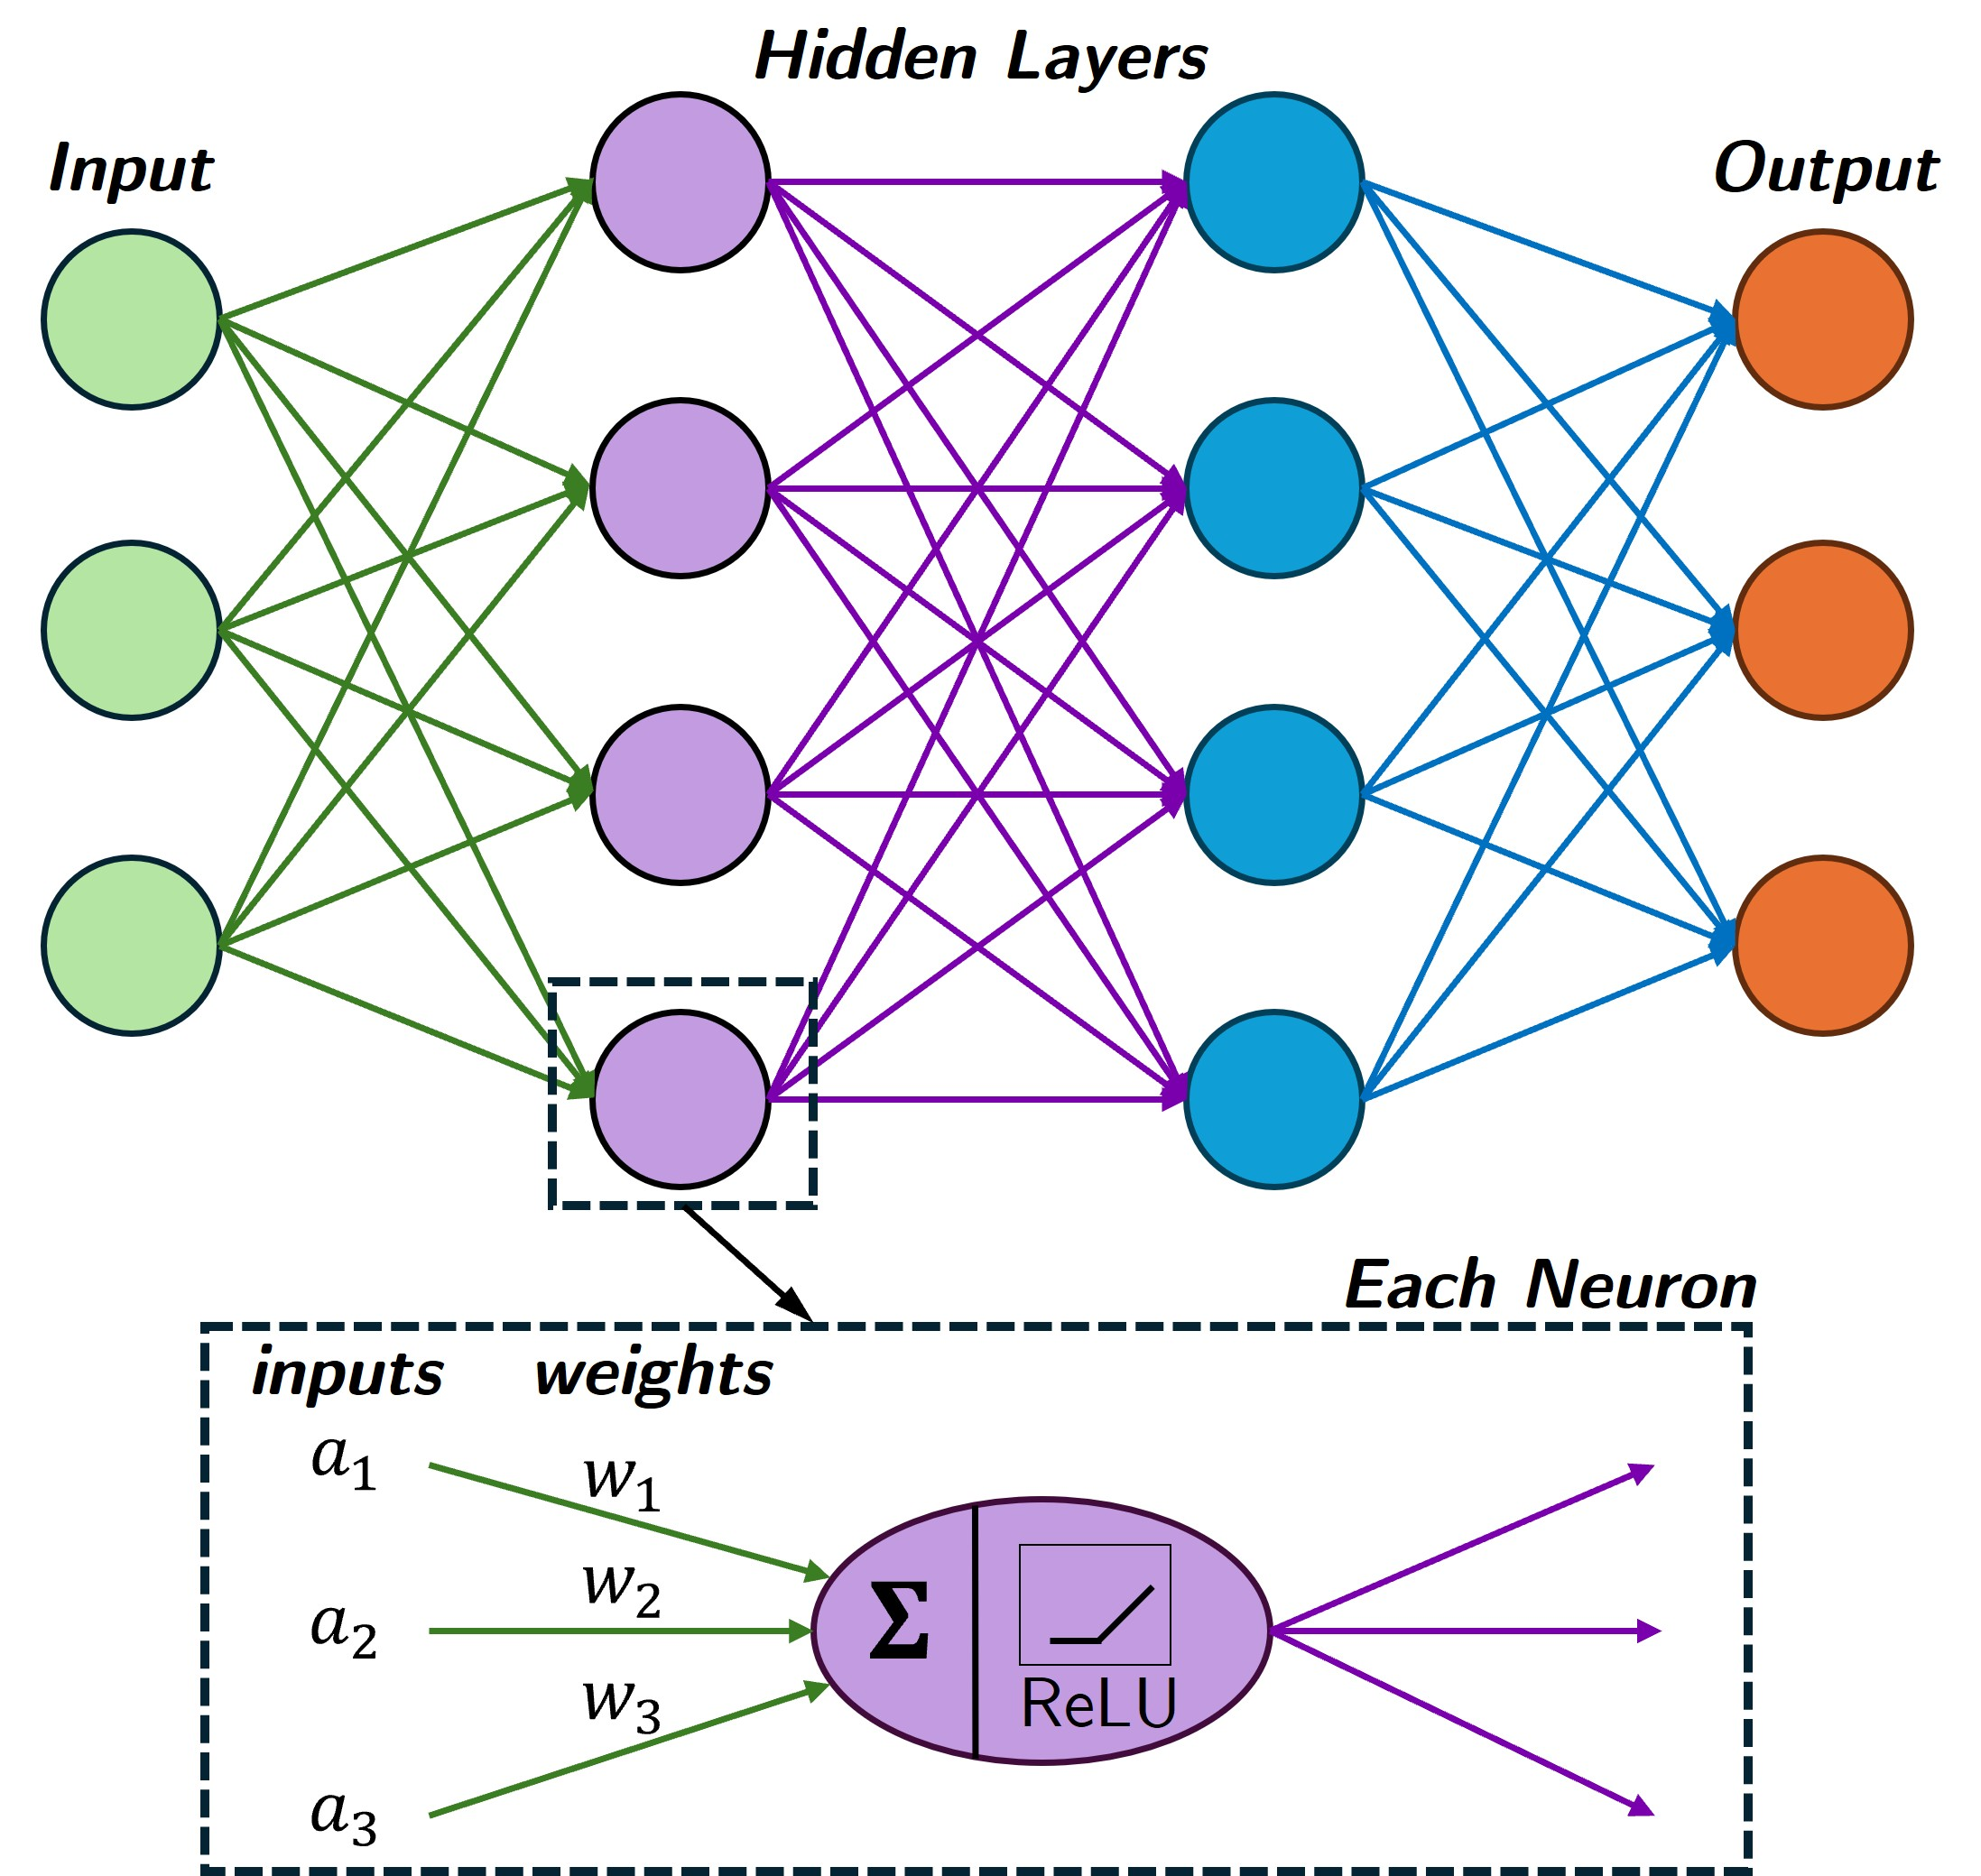
\includegraphics[width=\textwidth]{images/NeuralNetwork.jpg}
			\end{figure}
    		\end{minipage}

	\vfill
	\vspace{0.65cm}
    	{\footnotesize\textcolor{gray}{\textit{Aydinoglu, A., Fazlyab, M., Morari, M., \& Posa, M. Stability Analysis of Complementarity Systems with Neural Network Controllers, ACM. 2021; 19: 1-10.}}}
	%\end{block}
\end{frame}

\begin{frame}{Neural ODEs}
	\begin{block}{Definition}
		\vspace{2mm}
		\begin{minipage}{0.47\textwidth}
			\begin{itemize}
				\item A neural network $\phi$ describes the time-derivatives of the state variables [Chen et al. [2018]].
					\begin{equation*}
						\frac{dx}{dt}(t) = \phi(x(t))
					\end{equation*}
				\item Computed using finite-step discrete approximations like the Euler method.
			\end{itemize}
		\end{minipage}
		\begin{minipage}{0.50\textwidth}
        		\centering
        		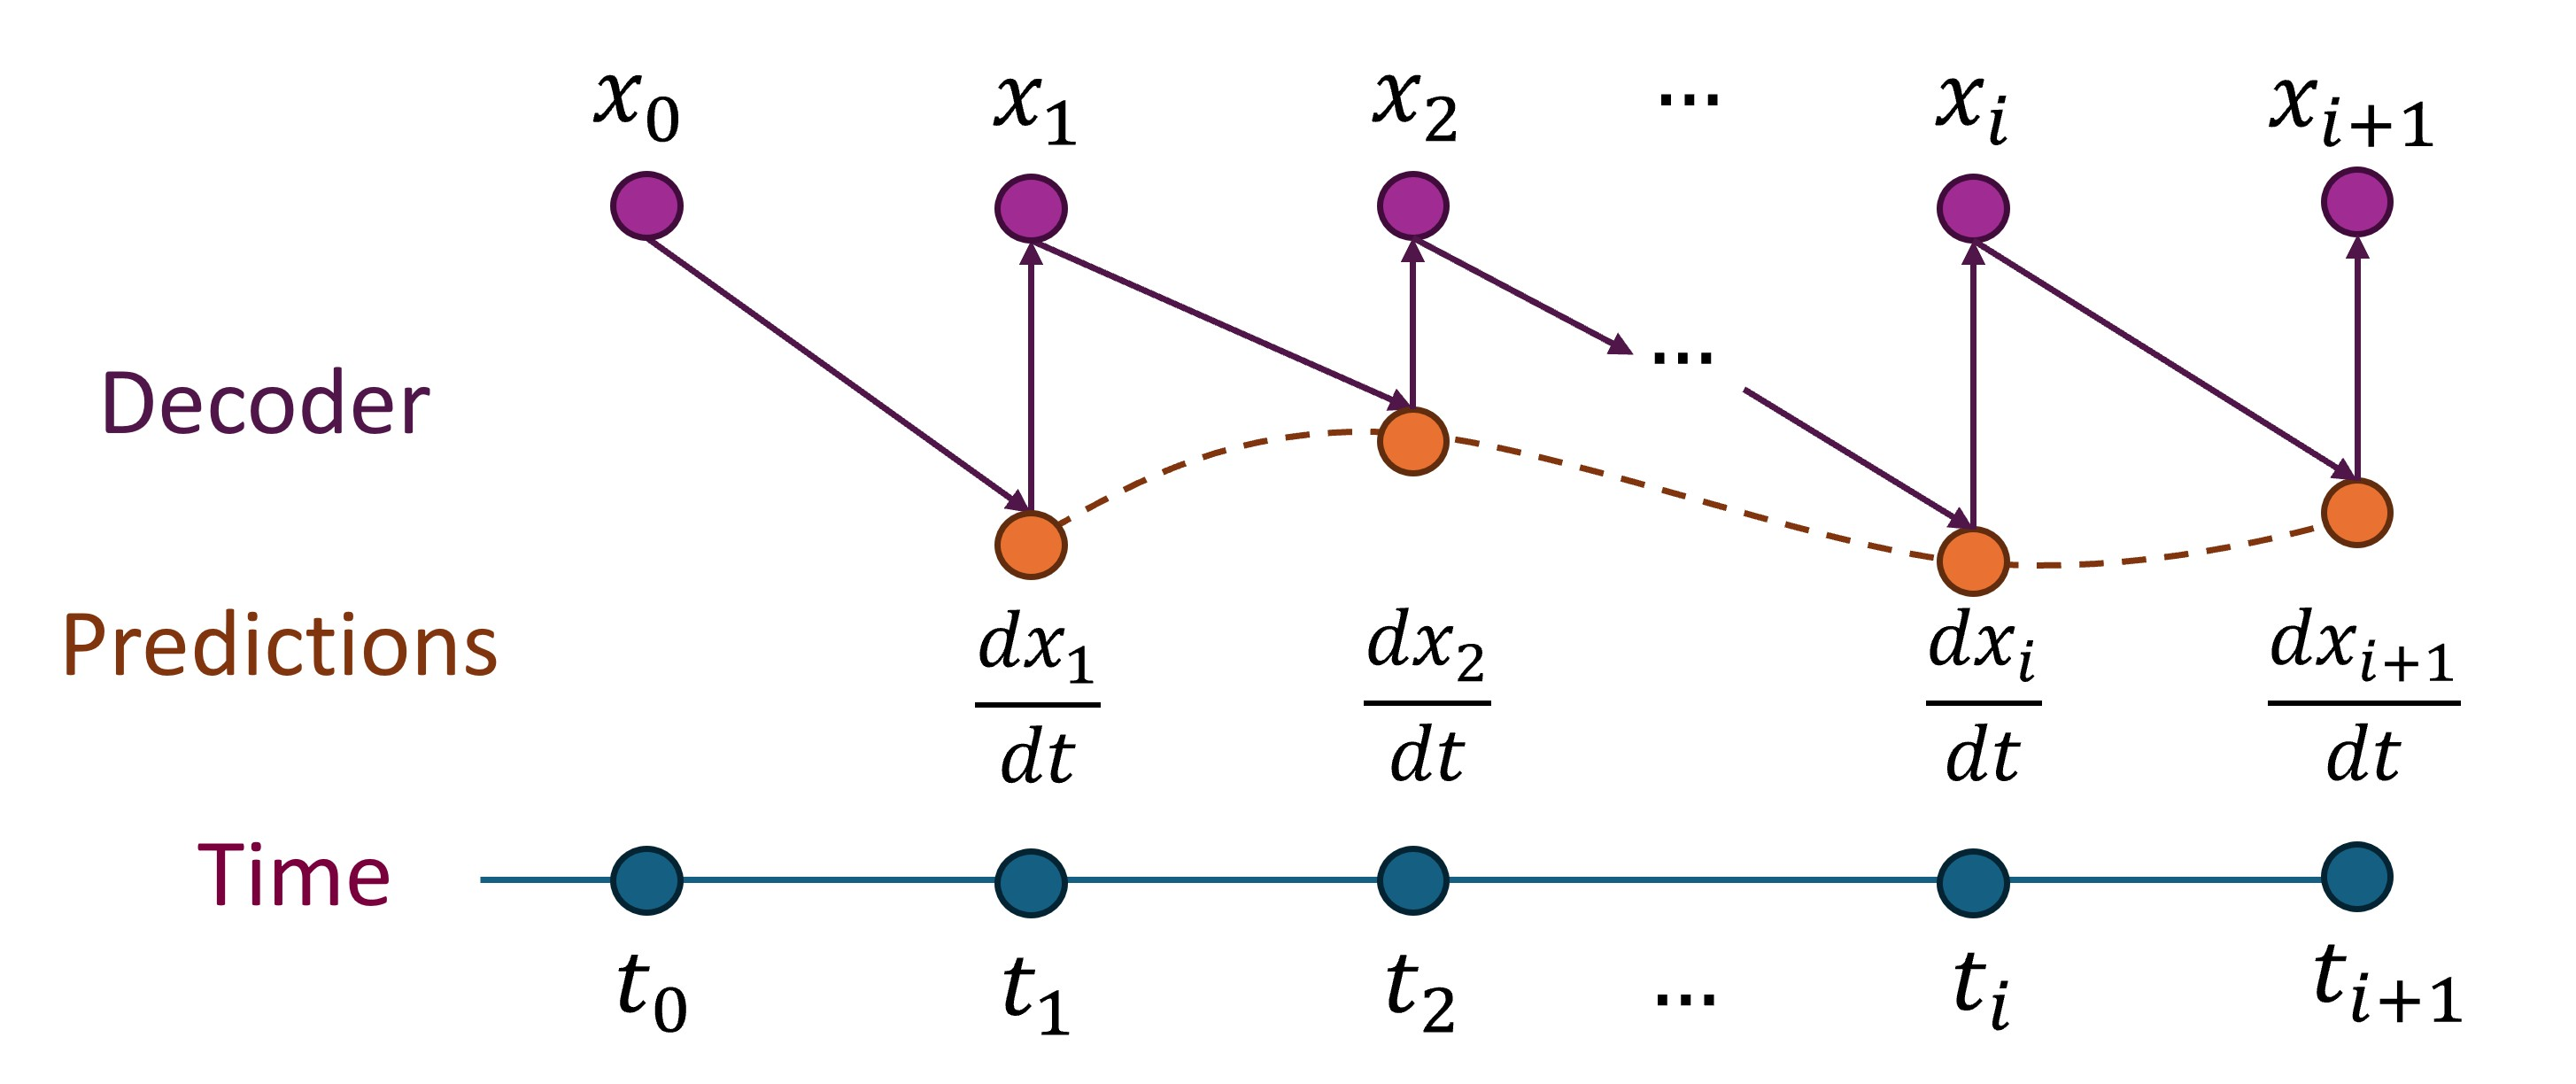
\includegraphics[width=\textwidth]{images/NeuralODE.jpg}
    		\end{minipage}
	\end{block}
\end{frame}

\subsection{Abs-normal forms}
\begin{frame}{Abs-normal forms}
\framesubtitle{Griewank et al., \emph{Linear Algebra Appl.} (2015)}
%Griewank et al., \emph{Math. Program.} (2016)
%Griewank et al., \emph{Linear Algebra Its Appl.} (2015)
\begin{block}{Definition}
    Given a continuous piecewise-affine function: %\f:\reals^n\to\reals^m$ 
    \[
        \f:\reals^n\to\reals^m,
    \]
    there exist matrices:
    \[
    \Z\in\reals^{s\times n}, \quad \J\in\reals^{m\times n}, \quad
    \Y\in\reals^{m\times s}, \quad
    \LL\in\reals^{s\times s}\; \text{(strictly lower triangular),}
    \] 
    and vectors:
    \[
    \cc \in\reals^s, \quad \bb\in\reals^m,
    \]
    such that, for any $\x\in\reals^n$, there is a unique vector $\z \in \reals^s$ satisfying:
    \[
    \begin{bmatrix}
      \z \\ \f(\x)
    \end{bmatrix}
    =
    \begin{bmatrix}
      \cc \\ \bb
    \end{bmatrix}
    +
    \begin{bmatrix}
      \Z & \LL \\ \J & \Y
    \end{bmatrix}
    \begin{bmatrix}
      \x \\ |\z|
    \end{bmatrix}.
    \]
This representation is an abs-normal form of $f$.
\end{block}
\vspace{-3mm}
\begin{block}{Observations}
\vspace{-1mm}
    \begin{itemize}      
        \item $\z$'s components are the arguments of the absolute value operations in $f$.
        %\item The right-hand side is called an abs-normal form of $f$.        
    \end{itemize}
\end{block}
\end{frame}

\begin{frame}{Construction example}
	%%%%%%%%%%%%%%%%
	 \only<1>{
		\begin{itemize}
		    \item A forward automatic-differentiation like procedure
		    \item Consider the piecewise-affine mapping:
		    \[
		        f(x)= x + \Big|2|3x + 4| - 5\Big| + 6|7x-8|,
		    \]
		    \item Construct the abs-normal form for $f$:
		    \begin{enumerate}
		        \item Define a vector $\z \in \reals^s$ for which:
		          \begin{align*}
		            z_1 &:= 3x + 4, \\
		            z_2 &:= 2|3x+4| - 5 = 2|z_1|-5, \\
		            z_3 &:= 7x-8.
		          \end{align*}
		         %whose components are the arguments of the absolute-value operations in $f$'s definition,
		         \item Express $f$ in terms of $x$ and $|\z|$:
			        \[
			            f(x) = x + |z_2| + 6|z_3|.
			        \]
		        \item The abs-normal form for $f$ is:
			        \[
			        \begin{bmatrix}
			          z_1 \\ z_2 \\ z_3 \\ f(x)
			        \end{bmatrix}
			        =
			        \begin{bmatrix}
			        \phantom{-}4 \\ -5 \\ -8 \\
			        \phantom{-}0
			        \end{bmatrix} 
			        +
			        \begin{bmatrix}
			          3 & 0 & 0 & 0 \\
			          0 & 2 & 0 & 0 \\
			          7 & 0 & 0 & 0 \\
			          1 & 0 & 1 & 6
			        \end{bmatrix}
			        \begin{bmatrix}
			          x \\ |z_1| \\ |z_2| \\ |z_3|
			        \end{bmatrix}.
			        \]
	  }

	%%%%%%%%%%%%
        \only<2>{
		\begin{itemize}
		    \item A forward automatic-differentiation like procedure
		    \item Consider the piecewise-affine mapping:
		    \[
		        f(x)= x + \Big|2|3x + 4| - 5\Big| + 6|7x-8|,
		    \]
		    \item Construct the abs-normal form for $f$:
		    \begin{enumerate}
		        \item Define a vector $\z \in \reals^s$ for which:
		          \begin{align*}
		            z_1 &:= 3x + 4, \\
		            z_2 &:= 2|3x+4| - 5 = 2|z_1|-5, \\
		            z_3 &:= 7x-8.
		          \end{align*}
		         %whose components are the arguments of the absolute-value operations in $f$'s definition,
		         \item Express $f$ in terms of $x$ and $|\z|$:
			        \[
			            f(x) = x + |z_2| + 6|z_3|.
			        \]
		        \item The abs-normal form for $f$ is:
			        \[
			        \begin{bmatrix}
			          z_1 \\ z_2 \\ z_3 \\ f(x)
			        \end{bmatrix}
			        =
			        \begin{bNiceMatrix}
			        \CodeBefore
			          \rectanglecolor{blue!25}{4-1}{4-4}
			          \rectanglecolor{green!25}{1-1}{3-3}
			        \Body  
			        % $\phantom{-}4$ \\
			        % $-5$ \\
			        % $-8$ \\
			        % $\phantom{-}0$
			        \phantom{-}4 \\ -5 \\ -8 \\
			        \phantom{-}0
			        \end{bNiceMatrix} 
			        +
			        \begin{bNiceMatrix}
			        \CodeBefore
			        \rectanglecolor{mcmastergrey!40}{1-1}{3-1}
			        \rectanglecolor{red!40}{1-2}{3-4}
			        \rectanglecolor{orange!30}{4-1}{4-1}
			        \rectanglecolor{purple!25}{4-2}{4-4}
			        \Body 
			          3 & 0 & 0 & 0 \\
			          0 & 2 & 0 & 0 \\
			          7 & 0 & 0 & 0 \\
			          1 & 0 & 1 & 6
			        \end{bNiceMatrix}
			        \begin{bmatrix}
			          x \\ |z_1| \\ |z_2| \\ |z_3|
			        \end{bmatrix}.
        			  \]
				  %%%%%%%%
				    \[
				    \begin{bmatrix}
				      \z \\ \f(\x)
				    \end{bmatrix}
				    =
				    \begin{bNiceMatrix}
					\CodeBefore
					      \rectanglecolor{blue!25}{2-1}{2-1}
				           \rectanglecolor{green!25}{1-1}{1-1}
					\Body
				           \cc \\ \bb
				    \end{bNiceMatrix}
				    +
				    \begin{bNiceMatrix}
					\CodeBefore
					        \rectanglecolor{mcmastergrey!40}{1-1}{1-1}
					        \rectanglecolor{red!40}{1-2}{1-2}
					        \rectanglecolor{orange!30}{2-1}{2-1}
					        \rectanglecolor{purple!25}{2-2}{2-2}
					\Body
				           \Z & \LL \\ \J & \Y
				    \end{bNiceMatrix}
				    \begin{bmatrix}
				      \x \\ |\z|
				    \end{bmatrix}.
				    \]
		}
		    \end{enumerate}
		\end{itemize}
\end{frame}

\begin{frame}{Construction for Neural Network}
\only<1>{
	\vspace{2mm}
	ReLU NNs are piecewise affine composite functions. Consolidate into a sequence of intermediate variables $\{\pmb{z}^{(\ell)} |\,\, \ell \in R^L\}$ for abs-normal form mapping. 
	\begin{block}{Piecewise affine mapping to abs-normal form for ReLU NN}
	\vspace{-1mm}
	\begin{figure}
	        \centering
	        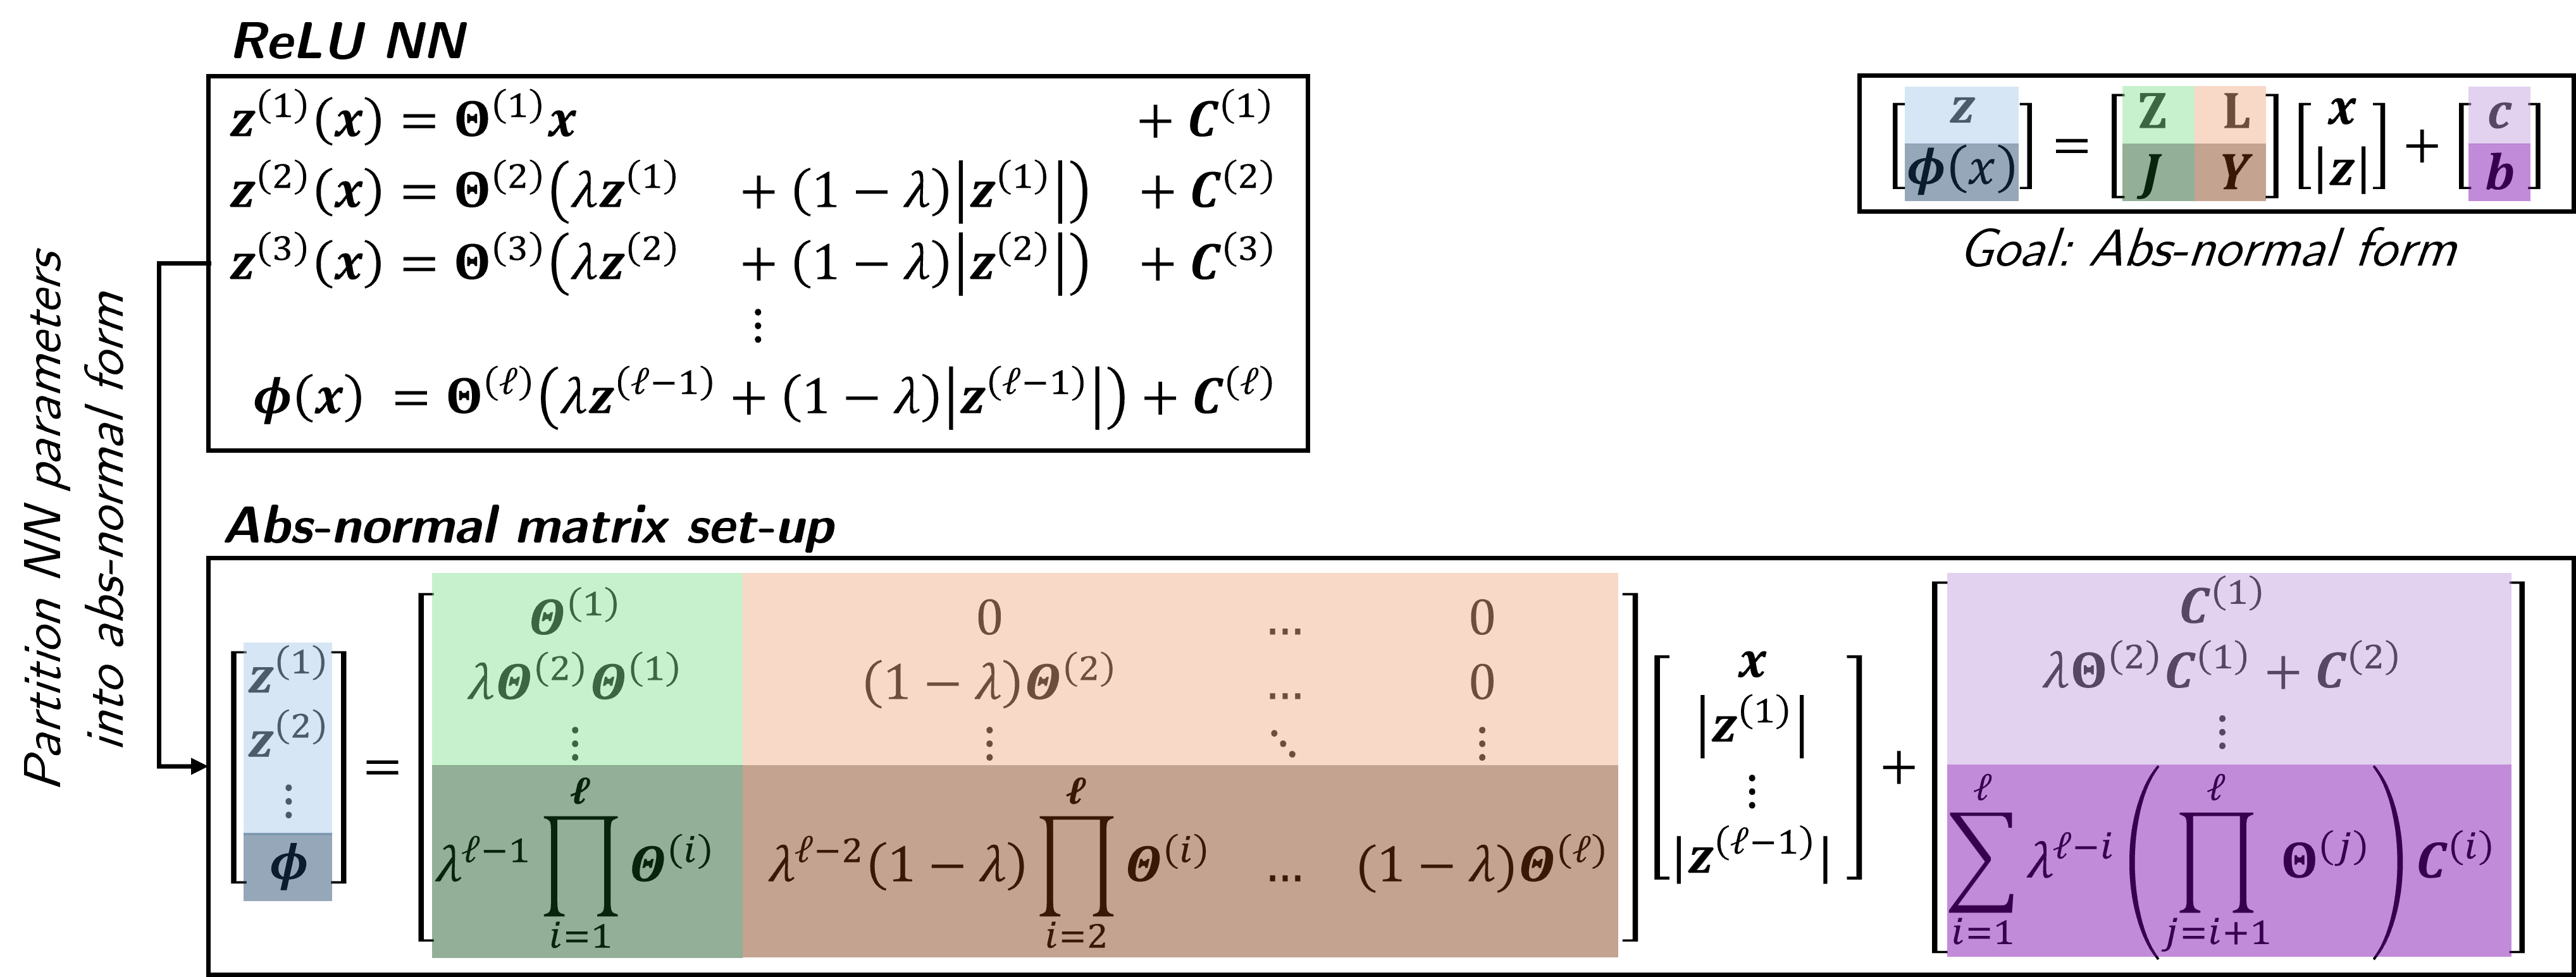
\includegraphics[width=1.0\textwidth]{images/Mapping_NN.png}
    	\end{figure}
	\end{block}
}

\only<2>{
\begin{block}{Calculating abs-normal form coefficients}
\begin{itemize}
		\item Griewank \& Walther (2018) describes a similar formulation for ReLU NNs which relies on the abs-linear form.
		\item Formula was (i) adapted to abs-normal form and (ii) to include NN bias parameters and alternative activation functions. 

	\begin{equation*}
		\mathbf{M\,z} =\bm{\zeta} \begin{bmatrix} \mathbf{x} \\ |\mathbf{z}|\end{bmatrix} +  \mathbf{C}
	\end{equation*}
	
	%\vspace{-3mm}
	\scalebox{0.75}{$\displaystyle
		\begin{bmatrix}
			I & 0 & \cdots & 0 & 0 \\
			-\lambda \bm{\Theta}^{(2)} & I & \cdots & 0 & 0 \\
			0 & - \lambda \bm{\Theta}^{(3)} & \cdots & 0 & 0 \\
			\vdots & \vdots & \ddots & \vdots & \vdots \\
			0 & 0 & \cdots & I & 0 \\
			0 & 0 & \cdots & -\lambda \bm{\Theta}^{(s+1)} & I
		\end{bmatrix}
		\begin{bmatrix}
			z_1 \\ z_2 \\ z_3 \\ \vdots \\ z_s \\ z_{s+1}
		\end{bmatrix}
		=
		\begin{bmatrix}
			\bm{\Theta}^{(1)} & 0 & 0 & \cdots & 0\\
			0 & (1-\lambda) \bm{\Theta}^{(2)} & 0 & \cdots & 0 \\
			0 & 0 & (1-\lambda) \bm{\Theta}^{(3)} & \cdots & 0 \\
			\vdots & \vdots & \vdots & \ddots & \vdots\\
			0 & 0 & 0 & \cdots & 0 \\
			0 & 0 & 0 & \cdots & (1-\lambda) \bm{\Theta}^{(s+1)} 
		\end{bmatrix}
		\begin{bmatrix}

			|z_1| \\ |z_2| \\ |z_3| \\ \vdots \\ |z_s| \\ |z_{s+1}|
		\end{bmatrix}
		+
		\begin{bmatrix}
			\mathbf{C}^{(1)} \\ \mathbf{C}^{(2)} \\ \mathbf{C}^{(3)} \\ \vdots \\ \mathbf{C}^{(s)} \\ \mathbf{C}^{(s+1)}
		\end{bmatrix}
    $}

	\vspace{2mm}
	where $\lambda = \tfrac{1}{2}$ for regular ReLU and $\lambda = \frac{1 + \alpha}{2}$ for leaky ReLU. 

\end{itemize}
\end{block}
}
\end{frame}

\subsection{Complementary Problems}
\begin{frame}{Complementary Problems}
	\begin{itemize}
		\item Variables $x$ and $y$ are \textbf{complementary} to each other if the following hold:
		\begin{enumerate}
			\item $\mathbf{x \geq 0}$		\vspace{2mm}
			\item $\mathbf{y \geq 0}$		\vspace{2mm}
			\item $\mathbf{x^T y = 0}$	\vspace{0.5mm}
		\end{enumerate}
		\item \textbf{Notation}: Written compactly as $\mathbf{0 \leq x \perp y \geq 0}$. 
		\vspace{2mm}
		\item \textbf{Linear Complementary Problem} (LCP): Find $\mathbf{x}$ such that:
			\begin{align*}
				\mathbf{0 \leq x \perp Ax + b \geq 0}
			\end{align*}
		\item \textbf{Mixed Linear Complementary Problem} (MLCP): For problems with both (i) complementary variable $\mathbf{x}$ and (ii) free variable $\mathbf{z}$:
			\begin{align*}
				\mathbf{Ax - Bz + a = 0} \\ 
				\mathbf{0 \leq x \perp Cx + Dz + b\geq 0}
			\end{align*}
	\end{itemize}
\end{frame}

%\subsection{Established root-finding approach}
%\begin{frame}{Established root-finding approach}
%\framesubtitle{Griewank et al., \emph{Linear Algebra Its Appl.} (2015)}  
%\begin{itemize}
%    \item Consider a piecewise-affine function $f: \reals^n \rightarrow \reals^m$ in abs-normal form:
%    \[
%    \begin{bmatrix}
%      \z \\ \f(\x)
%    \end{bmatrix}
%    =
%    \begin{bmatrix}
%      \cc \\ \bb
%    \end{bmatrix}
%    +
%    \begin{bmatrix}
%      \Z & \LL \\ \J & \Y
%    \end{bmatrix}
%    \begin{bmatrix}
%      \x \\ |\z|
%    \end{bmatrix}.
%    \]
%    \item Assume:
%    \[
%        \alert{m=n} \qquad \text{and} \qquad \alert{\J\;\; \text{is nonsingular.}}
%    \]
%    \item Define:
%    \[
%    \bS:=\LL-\Z\J^{-1}\Y\in\reals^{s\times s},
%    \qquad
%    \hat{\cc}:=\cc-\Z\J^{-1}\bb\in\reals^s.
%    \]
%    \item Then, $\f(\x)=\0$ solves the following mixed linear complementarity problem (MLCP):
%    \[
%    \begin{array}{rcl}
%    \uu-\w&=&\hat{\cc} + \bS(\uu+\w) \\
%    \0\leq \uu &\perp& \w\geq \0,
%    \end{array}
%    \]
%    where $\uu \in \reals^s:= \max(\0,\z)$ and $\w \in \reals^s:= \max(\0,-\z)$ (componentwise).
%    \item If $(\I-\bS)$ is nonsingular, $\w$ solves the following linear complementarity problem (LCP):
%    \[
%      \0\leq (\I-\bS)^{-1}\hat{\cc} + (\I-\bS)^{-1}(\I+\bS)\w\perp \w\geq \0,
%    \]
%    \item Complementarity-based solvers, like PATH, are powerful in practice
%    %\item Future complementarity-based solvers can be effectively adapt to piecewise-affine functions
%\end{itemize}
%\end{frame}

\section{New results concerning piecewise-affine functions}

\subsection{New root-finding and optimization approaches}
\begin{frame}{New root-finding approach}
\framesubtitle{Zhang \& Khan, \emph{AD 2024}} 
\only<1>{
\begin{block}{New MLCP formulation}
\begin{itemize}
    \item Since $\LL$ is strictly lower triangular, $(\I - \LL)$ is unit lower triangular and invertible
    \item Define matrices and vectors:
        \begin{align*}
        \tilde{\cc}&:=(\I-\LL)^{-1}\cc, &
        \tilde{\bb}&:= \bb+\Y\tilde{\cc}, &
        \tilde{\LL}&:= (\I-\LL)^{-1}(\I+\LL),\\
        \tilde{\Y}&:= \Y(\I+\tilde{\LL}),& 
        \tilde{\Z}&:= (\I-\LL)^{-1}\Z,& 
        \tilde{\J}&:= \J+\Y\tilde{\Z}.
      \end{align*}
    \item $\f(\x)=\0$ solves the following MLCP:
    \[
    \begin{array}{rcl}
      \0 &=& \tilde{\bb} + \tilde{\J}\x + \tilde{\Y}\w \\
      \0\leq \w &\perp& \tilde{\cc} + \tilde{\Z}\x + \tilde{\LL}\w \geq \0.
    \end{array}
    \]
    where $\w \in \reals^s:= \max(\0,-\z)$. 
    \vspace{-2mm}
\end{itemize}
\end{block}
\vspace{-2mm}
\begin{block}{Properties}
\begin{itemize}
    \item Fewer variables, and fewer equations than previous MLCP (per Griewank et. al, 2015)
    \item No requirement that $m=n$ or nonsingular $\tilde{\J}$ 
    \item Compatible with PATH solver 
\end{itemize}
\end{block}

}

\only<2>{
\begin{block}{New LCP formulation}
    \begin{itemize}
        \item If $m=n$ and $\tilde{\J}$ is nonsingular, define:
          \[
            \pmb{\sigma}:=\tilde{\cc} - \tilde{\Z}\tilde{\J}^{-1}\tilde{\bb},
            \qquad
            \pmb{\rho}:=\tilde{\LL} - \tilde{\Z}\tilde{\J}^{-1}\tilde{\Y}.
          \]
        \item $\f(\x)=\0$ can be obtained via:
        \[
            \tilde{\J}\x=-\tilde{\bb}-\tilde{\Y}\w,
        \]
        where $\w \in \reals^s$ solves the LCP:
        \[
        \0\leq \w \perp \pmb{\sigma} + \pmb{\rho} \w \geq \0.
        \]
    \end{itemize}
\end{block}
\begin{block}{Properties}
\begin{itemize}
    \item From our experience, $\tilde{\J}$ seems to be nonsingular when each $|z_i|$ contributes meaningfully to $f$
    \item Fewer variables than both MLCP formulations
    \item More suited to PATH solver 
\end{itemize}
\end{block}

}
\end{frame}

\begin{frame}{New optimization approach}
\framesubtitle{Zhang \& Khan, \emph{AD 2024}} 
\begin{itemize}\setlength{\itemsep}{5pt}
    \item Consider a piecewise-affine function $f: \reals^n \rightarrow \reals$ in abs-normal form:
    \[
    \begin{bmatrix}
      \z \\ f(\x)
    \end{bmatrix}
    =
    \begin{bmatrix}
      \cc \\ \bb
    \end{bmatrix}
    +
    \begin{bmatrix}
      \Z & \LL \\ \J & \Y
    \end{bmatrix}
    \begin{bmatrix}
      \x \\ |\z|
    \end{bmatrix}.
    \]
    \item Minimizing $f(\x)$ is equivalent to solving a linear program with complementarity constraints (LPCC):
    \[
    \begin{array}{cl}
      \displaystyle \min_{\x\in\reals^n,\w\in\reals^s} & \tilde{b} + \tilde{\J}\x + \tilde{\Y}\w \medskip\\
      \mathrm{s.t.} & \0 \leq \w\perp\tilde{\cc} + \tilde{\Z}\x + \tilde{\LL}\w\geq \0.
    \end{array}
    \]
    \begin{itemize}\setlength{\itemsep}{3pt}
        \item can be solved using Branch-and-Cut [Yu et al. \emph{Math. Program. Comput. (2019)}]
        %\item or, if bounds on $\x^\star$ and $\w^\star$ are known, we can rewrite LPCC as a MILP
    \end{itemize}
    \item If bounds on $\x^\star$ and $\w^\star$ are known, we can rewrite LPCC as a MILP using ``big-M'':
    %\item The following MILP is a standard ``big-M'' reformulation of the LPCC:
    \[
    \begin{array}{cl}
      \displaystyle \min_{\x,\w,\y}& \tilde{b} + \tilde{\J}\x + \tilde{\Y}\w
        \medskip \\
      \mathrm{s.t.} & \0 \leq \w \leq \mu \y, \\
      & \0 \leq \tilde{\cc} + \tilde{\Z}\x + \tilde{\LL}\w \leq \mu(\e-\y), \\
      & \y\in\{0,1\}^s.
    \end{array}
    \]
\end{itemize}
\end{frame}

\begin{frame}{Background: horizon function}
\begin{block}{Horizon function [Dontchev and Rockafellar, \emph{Set-Valued Analysis} (2004)]}

Given a continuous function $f:\reals^n\to\reals$, the horizon function for $f$ is the mapping:
\begin{align*}
  &f^\infty(\bm\xi) = \lim_{\delta\downTo{0}} 
    \left(\inf\{\lambda f(\tfrac{\x}{\lambda}):
      \quad 0<\lambda<\delta,\quad \|\x-\bm\xi\|<\delta\}\right).
\end{align*}
\end{block}
\vspace{-3mm}
\begin{block}{Example}
    \begin{minipage}{0.55\textwidth}
        The horizon function \( f^\infty(x) \) of the following\\ piecewise-affine function:
        \[
            f(x) = x + \Big|2|x - 2| - 10\Big| + 20,    
        \]
    \end{minipage}
    \hfill
    \begin{minipage}{0.4\textwidth}
        \centering
        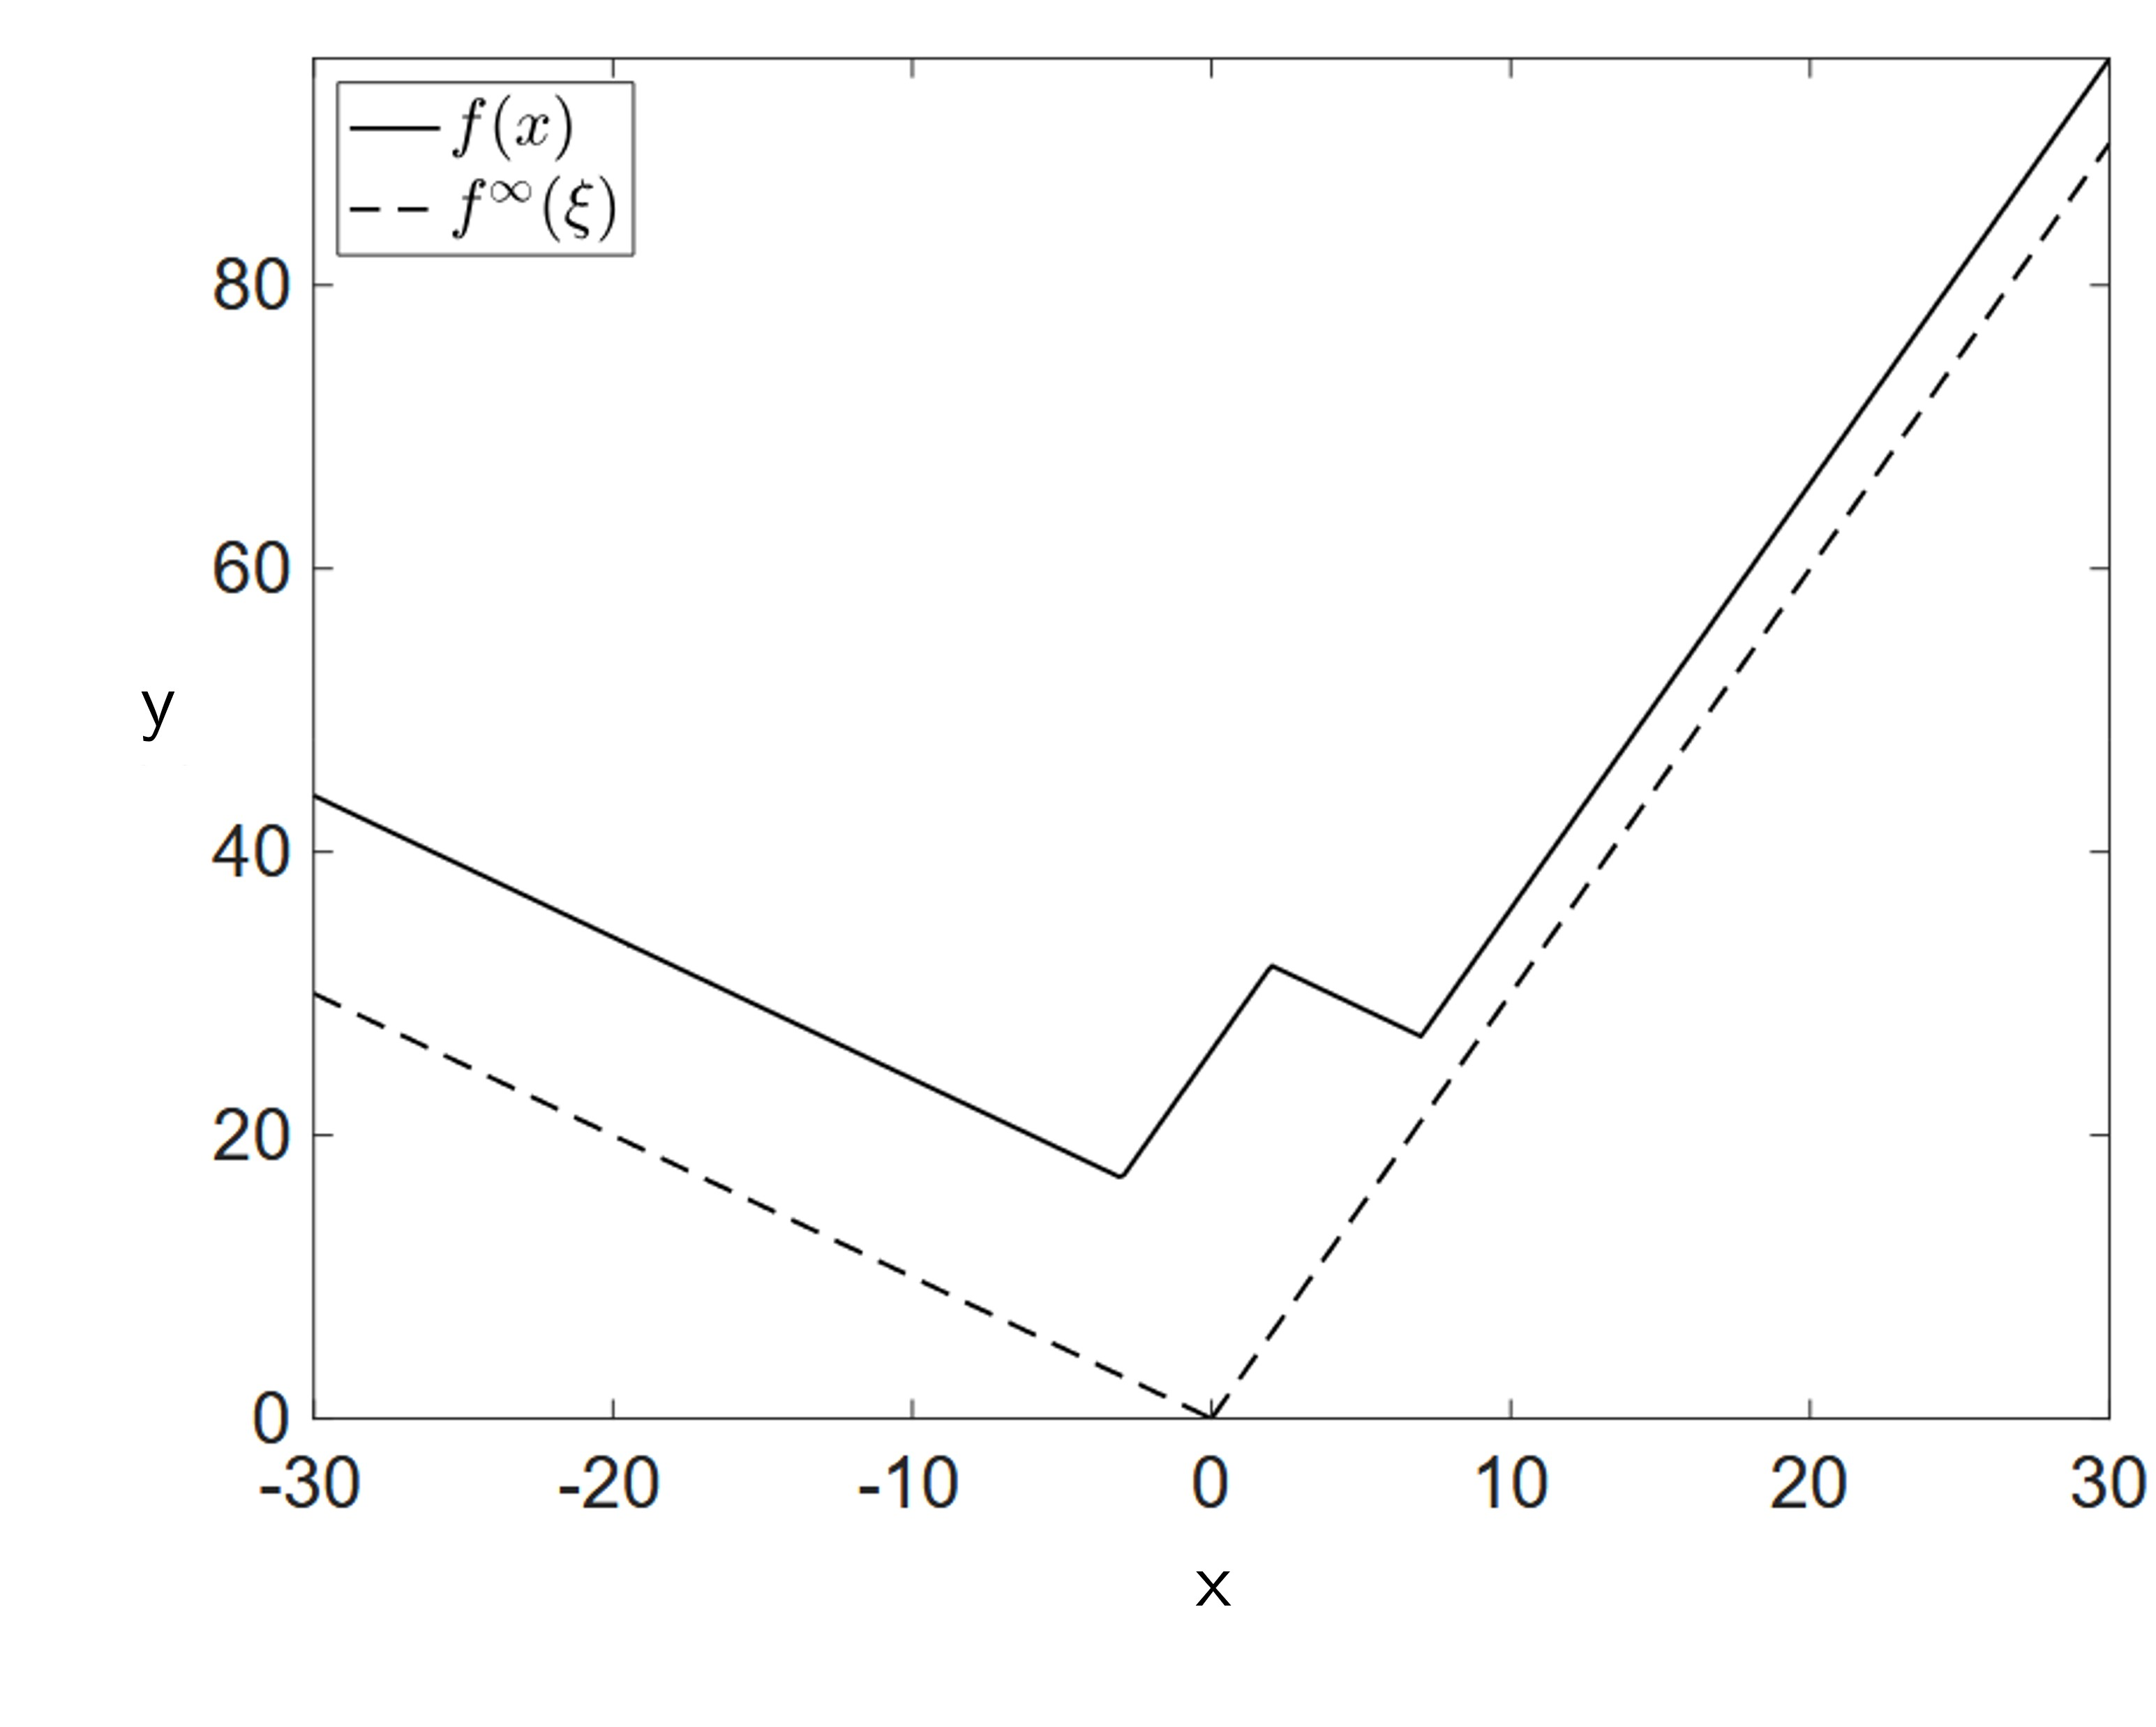
\includegraphics[width=\textwidth]{images/horizonfunction.jpg}
    \end{minipage}
\end{block}
\end{frame}

\begin{frame}{Existence of minima}
\framesubtitle{Zhang \& Khan, \emph{AD 2024}}  
\only<1>{%
	\begin{itemize}\setlength{\itemsep}{10pt}
		   \item Any horizon function $f^\infty$ has $\inf_{\bm\xi\in\reals^n}f^\infty(\bm\xi)\in\{-\infty,0\}$.
	        \item A global minimum exists if and only if  $\inf_{\bm\xi\in X}f^\infty(\bm\xi)=0$,
	        \item Then, if and only if $f^\infty(\bm\xi) + 1 = 0$ has no solution $\bm\xi\in\reals^n$,\\ a global minimum exists.
	\end{itemize}

	\begin{columns}
		\begin{column}{0.55\textwidth}
			\begin{figure}
		          \centering
		          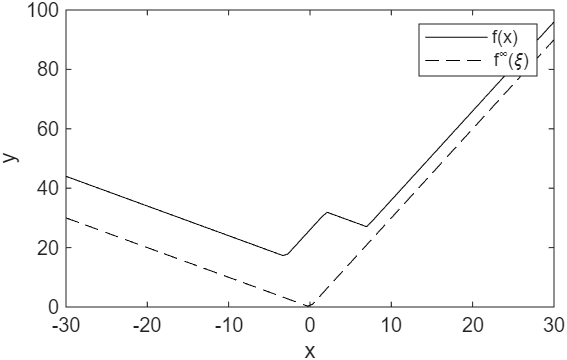
\includegraphics[height=0.4\textheight]{images/HorizonFuncFig1.png}
				\caption*{\textit{$\quad$Function with global minimum.}}
			\end{figure}
		\end{column}
		\begin{column}{0.45\textwidth}
			\begin{figure}
		          \centering
			     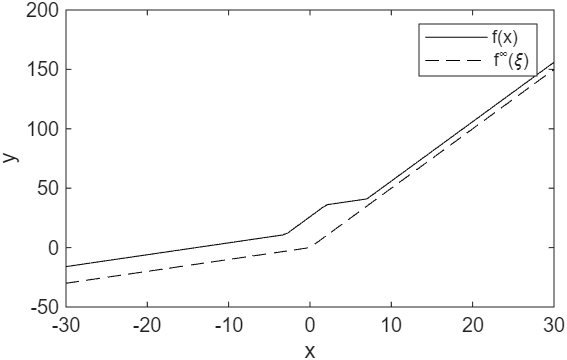
\includegraphics[height=0.41\textheight]{images/HorizonFuncFig2.png}
				\caption*{\textit{$\quad\quad$Function without global minimum.}}
			\end{figure}
		\end{column}
	\end{columns}
}

\only<2>{
\begin{itemize}\setlength{\itemsep}{5pt}
    \item How to solve $f^\infty(\bm\xi) + 1 = 0$?
    
    \item The horizon function $f^\infty$ is piecewise-linear, and has the abs-normal form:
    \[
    \begin{bmatrix}
      \bm\zeta \\ f^\infty(\bm\xi)
    \end{bmatrix}
    \equiv
    \begin{bmatrix}
      \Z & \LL \\ \J & \Y
    \end{bmatrix}
    \begin{bmatrix}
      \bm\xi \\ |\bm\zeta|
    \end{bmatrix},
    \]
    where $\bm\zeta/\bm\xi$ plays the same role as $\z/\x$ did.
    \item The following MLCP solves $f^\infty(\bm\xi) + 1 = 0$:   
    \[
    \begin{array}{rcl}
    0 &=& 1 + \tilde{\J}\bm\xi + \tilde{\Y}\bm\omega \\
    \0 \leq \bm\omega &\perp & \tilde{\Z}\bm\xi + \tilde{\LL}\bm\omega \ge \0,
    \end{array}
    \]
    where $\bm\omega \in \reals^s:= \max(\0,-\bm\zeta)$.
    \item MLCP characterizes existence of a global minimum for piecewise-affine functions.
    \item This enables verification of a global minimum before minimization.
\end{itemize}

}

\end{frame}

\subsection{Implementation and examples}
\begin{frame}{Implementation and examples}
\framesubtitle{Zhang \& Khan, \emph{AD 2024}} 
\only<1>{
  \vspace{1mm}
  \begin{itemize}
      \item Implemented in Julia v1.10.5
      \begin{itemize}
          \item MLCP and LCP solvers: PATHSolver.jl 1.7.5 and BARON.jl v0.8.3 in JuMP
          \item Input: four matrices and two vectors of the abs-normal form
      \end{itemize}
  \end{itemize}
  
  \begin{block}{Root-finding example}
    \begin{itemize}
    \item Consider a piecewise-affine function:
    \begin{align*}
        &f_1(x_1,x_2) = \Bigl|\left|x_1+2\right|+x_2-1\Bigr| - x_2 -1,\\
        &f_2(x_1,x_2) = \left|x_1+2\right| + 2x_2-1,
    \end{align*}
    with the abs-normal form:
    \[
    \begin{bmatrix}
      z_1 \\ z_2 \\ f_1 \\f_2
    \end{bmatrix}
    =
    \begin{bmatrix}
      \phantom{-} 2 \\ -1 \\ -1 \\ -1
    \end{bmatrix}
    +
    \begin{bmatrix}
      1 & 0 & 0 & 0 \\
      0 & 1 & 1 & 0 \\
      0 & -1 & 0 & 1 \\
      0 & 2 & 1 & 0 
    \end{bmatrix}
    \begin{bmatrix}
      x_1 \\ x_2 \\ |z_1| \\ |z_2|
    \end{bmatrix}.
    \]
    \item The root $(x_1,x_2)=(0,-0.5)$ was found using both the MLCP and the LCP formulations.
    \end{itemize}
  \end{block}
    }
\only<2>{
  \vspace{1mm}
  \begin{itemize}
      \item Implemented in Julia v1.10.5
      \begin{itemize}
          \item MLCP solver for verification: BARON.jl v1.7.5 in JuMP
          \item MILP and LPCC solver for minimization: BARON.jl v1.7.5 in JuMP
          \item Input: four matrices and two vectors of the abs-normal form
      \end{itemize}
  \end{itemize}

  \begin{block}{Optimization example}
    \begin{itemize}
    \item Objective: 
    \[
    f(x) = \Bigl|x_1+ \left|2x_2-1\right| \Bigr|+ \left|3 + x_3\right|,
    \] with the abs-normal form:
    \[
    \begin{bmatrix}
      z_1 \\ z_2 \\ z_3 \\ f(x)
    \end{bmatrix}
    =
    \begin{bmatrix}
      -1 \\ \phantom{-}0 \\ \phantom{-}3 \\ \phantom{-}0
    \end{bmatrix}
    +
    \begin{bmatrix}
      0 & 2 & 0 & 0 & 0 & 0 \\
      1 & 0 & 0 & 1 & 0 & 0\\
      0 & 0 & 1 & 0 & 0 & 0 \\
      0 & 0 & 0 & 0 & 1 & 1
    \end{bmatrix}
    \begin{bmatrix}
      x_1 \\ x_2 \\ x_3 \\ |z_1| \\ |z_2| \\ |z_3|
    \end{bmatrix}.
    \]
    \vspace{-5mm}
    \item The existence of a global minimum for $f(\x)$ was verified.
    \item The minimum is $\x^\ast=(0.0, 0.5, -3.0)$.
    \end{itemize}
  \end{block}
}
\end{frame}

\begin{frame}
\frametitle{Root-finding scaling experiment}
\framesubtitle{Zhang \& Khan, \emph{AD 2024}} 
\begin{columns}[t] % Aligns content at the top
    \begin{column}{0.45\textwidth}
        \begin{itemize}\setlength{\itemsep}{10pt}
		 \vspace{-2mm}
            \item Consider a randomly generated piecewise-affine function:
            \[
            f:\reals^n\to\reals^n
            \]
            in abs-normal form with $s=n$, where the coefficients\newline
            \begin{itemize}\setlength{\itemsep}{5pt}
                \item $\bb,\cc,\Y$ are generated based on a normal distribution and rounded to the nearest integers
                \item $\Z$ is identity matrix; $\J$ is zero matrix
                \item $\LL$ has ones on the first subdiagonal, with all other elements being zero
            \end{itemize}
        \end{itemize}
    \end{column}
    \begin{column}{0.55\textwidth}
    \begin{itemize}
	   \vspace{-2mm}
        \item The average CPU time (s) for solving $\f(\x)=\0$:
        \begin{itemize}
            \item PATH may fail to solve MLCP and LCP at larger $n$, BARON does not
            \item LCP outperforms MLCP; PATH outperforms BARON
        \end{itemize}
    \end{itemize}
    \vspace{-4mm}
        \begin{figure}
            \centering
            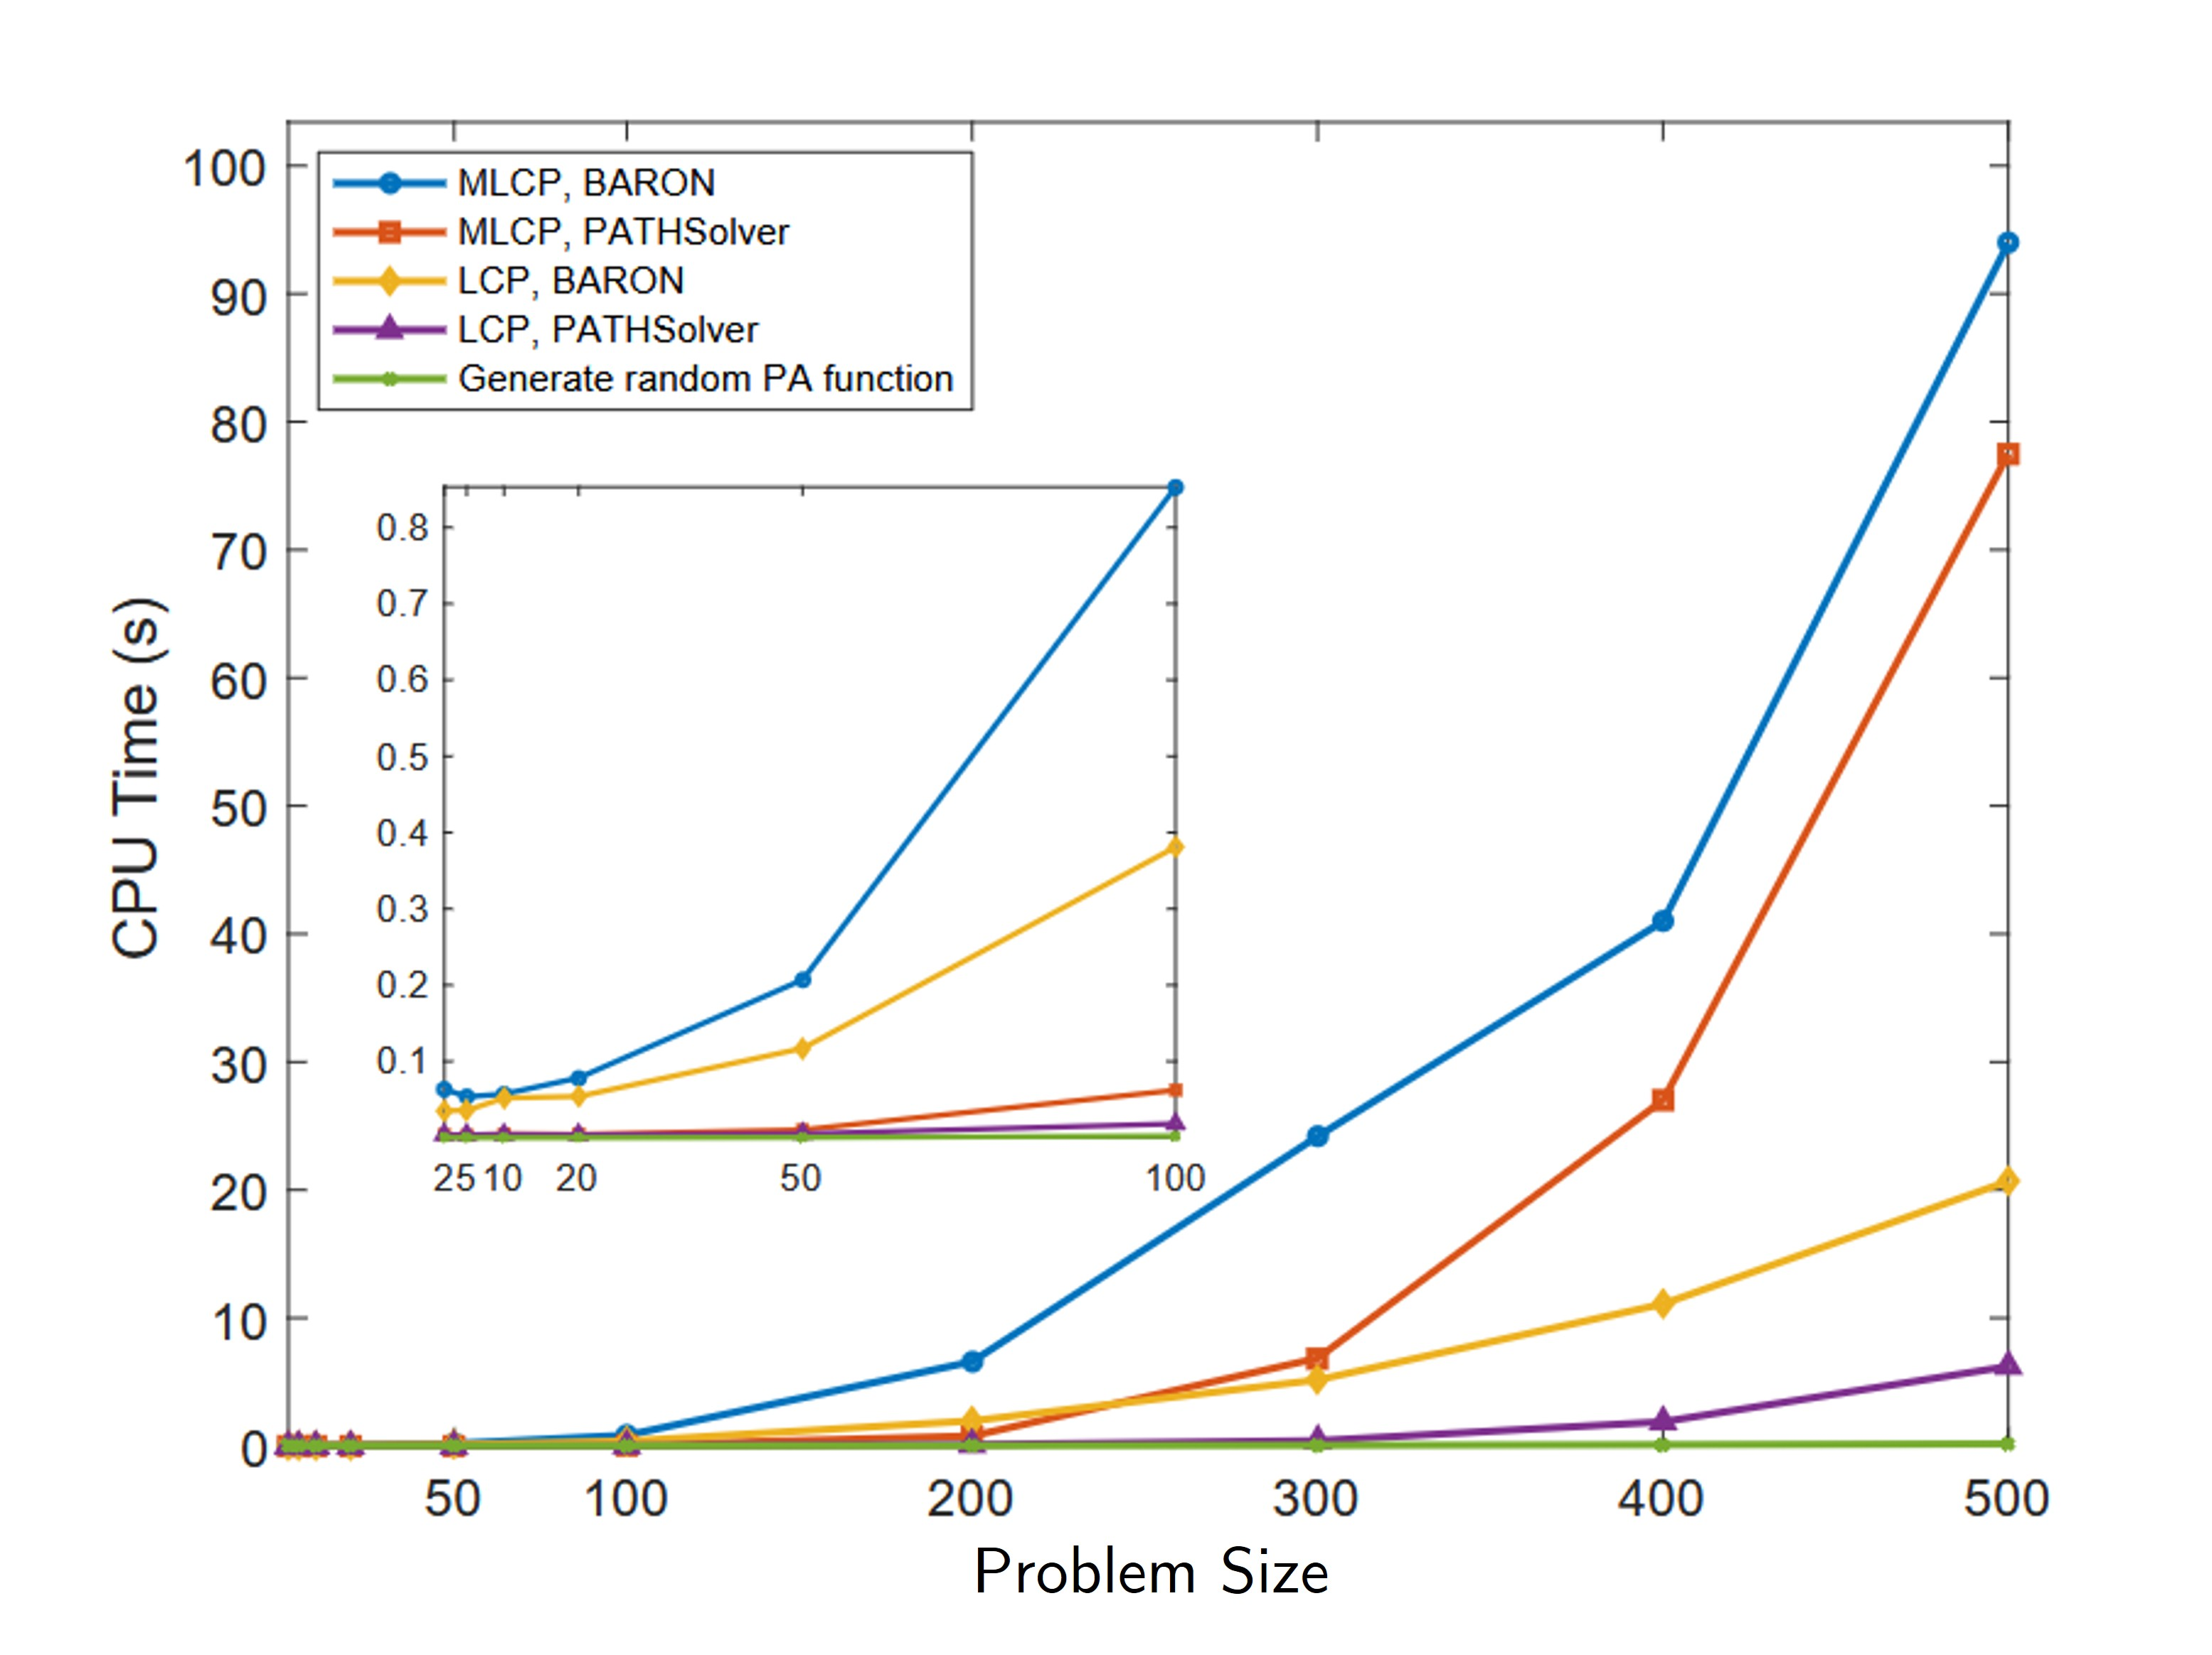
\includegraphics[width=1.0\textwidth]{images/Root_finding_S1.jpg}
        \end{figure}
        \vspace{-2mm}
    \end{column}
\end{columns}
\end{frame}


\begin{frame}
\frametitle{Root-finding scaling experiment}
\framesubtitle{Zhang \& Khan, \emph{AD 2024} \\
	Comparison with approach of Griewank et al. (2015)}
\begin{columns}[t]
    \begin{column}{0.45\textwidth}
    \begin{itemize}\setlength{\itemsep}{10pt}
	  \vspace{-2mm}
        \item Consider a randomly generated piecewise-affine function:
        \[
        f:\reals^n\to\reals^n
        \]
        in abs-normal form, where the coefficients\newline
        \begin{itemize}\setlength{\itemsep}{5pt}
            \item $\bb,\cc,\Y$ are generated based on a normal distribution and rounded to the nearest integers
            \item $\Z, \J$ are identity matrices; \alert{$\J$ has to be nonsingular}
            \item $\LL$ has ones on the first subdiagonal, with all other elements being zero
        \end{itemize}
        \item Griewank et al.'s MLCP can not be solved by PATH; BARON is used
    \end{itemize} 
    \end{column}
    \begin{column}{0.55\textwidth}
    \begin{itemize}
	  \vspace{-2mm}
        \item The average CPU time (s) for solving $\f(\x)=\0$:
            \begin{itemize}
        \item PATH may fail to solve $\f(\x)=\0$ when $n\ge100$
        \item For the same problem, our new LCP requires less CPU time
        \end{itemize}
    \end{itemize}
    \vspace{-4mm}
        \begin{figure}
        \centering
        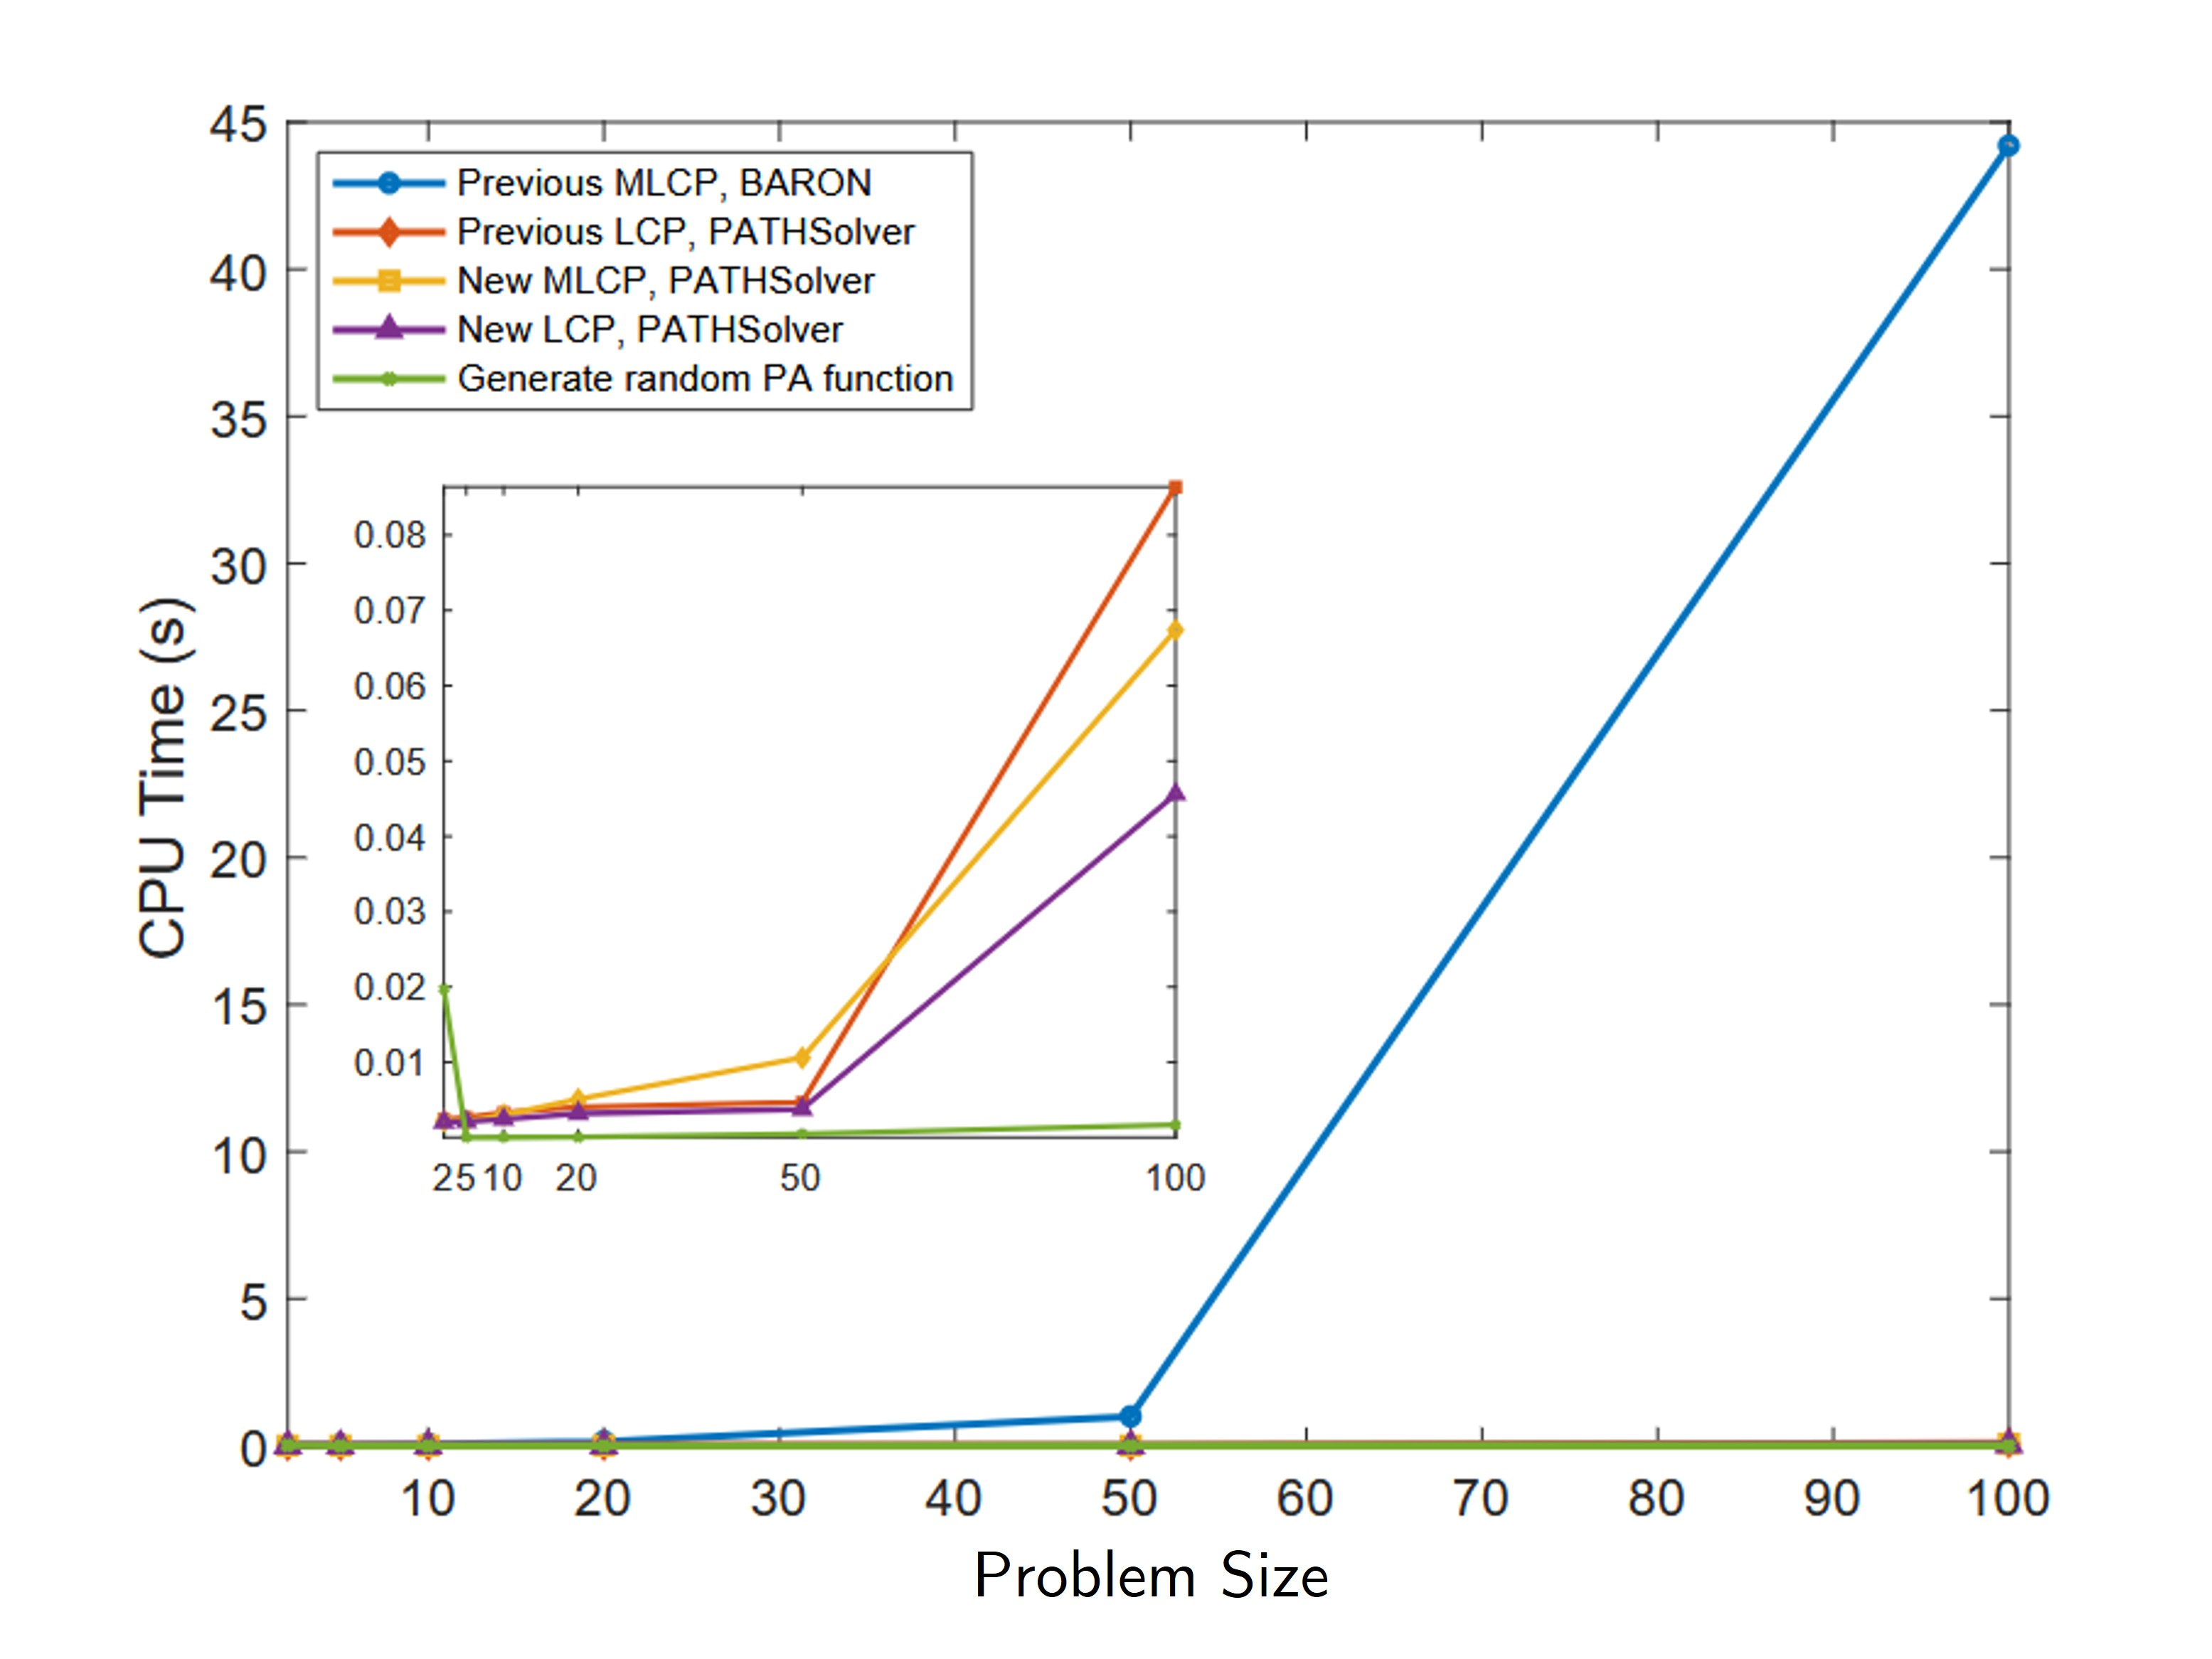
\includegraphics[width=1.0\textwidth]{images/Root_finding_S2.jpg}
    \end{figure}
    \end{column}
\end{columns}
\end{frame}

\begin{frame}
\frametitle{Optimization scaling experiment}
\framesubtitle{Zhang \& Khan, \emph{AD 2024}} 
\begin{columns}[t] % Aligns content at the top
    \begin{column}{0.45\textwidth}
        \begin{itemize}\setlength{\itemsep}{10pt}
            \item Consider a piecewise-affine function $f:\reals^n \rightarrow \reals$:
            \begin{align*}
              f(\x) &= \biggl| \bigl| |1000x_1| + 1000x_2 \bigr| + \dots + 1000x_n \biggr| \\
              &\qquad{}+ 1.0.
            \end{align*}
            in abs-normal form, where\newline
            \begin{itemize}\setlength{\itemsep}{5pt}
                \item $s=n$,
                \item the global minimum existence is verified using MLCP formulation
                \item before minimizing using MILP and LPCC formulations. 
            \end{itemize}
        \end{itemize}
    \end{column}
    
    \begin{column}{0.55\textwidth}
    \begin{itemize}
        \item The average CPU time (s) for minimizing $f(\x)$:
        \vspace{1mm}
        \begin{itemize}
            \item MILP is faster than LPCC for all $n$
        \end{itemize}
    \end{itemize}
    \vspace{-2mm}
        \begin{figure}
            \centering
            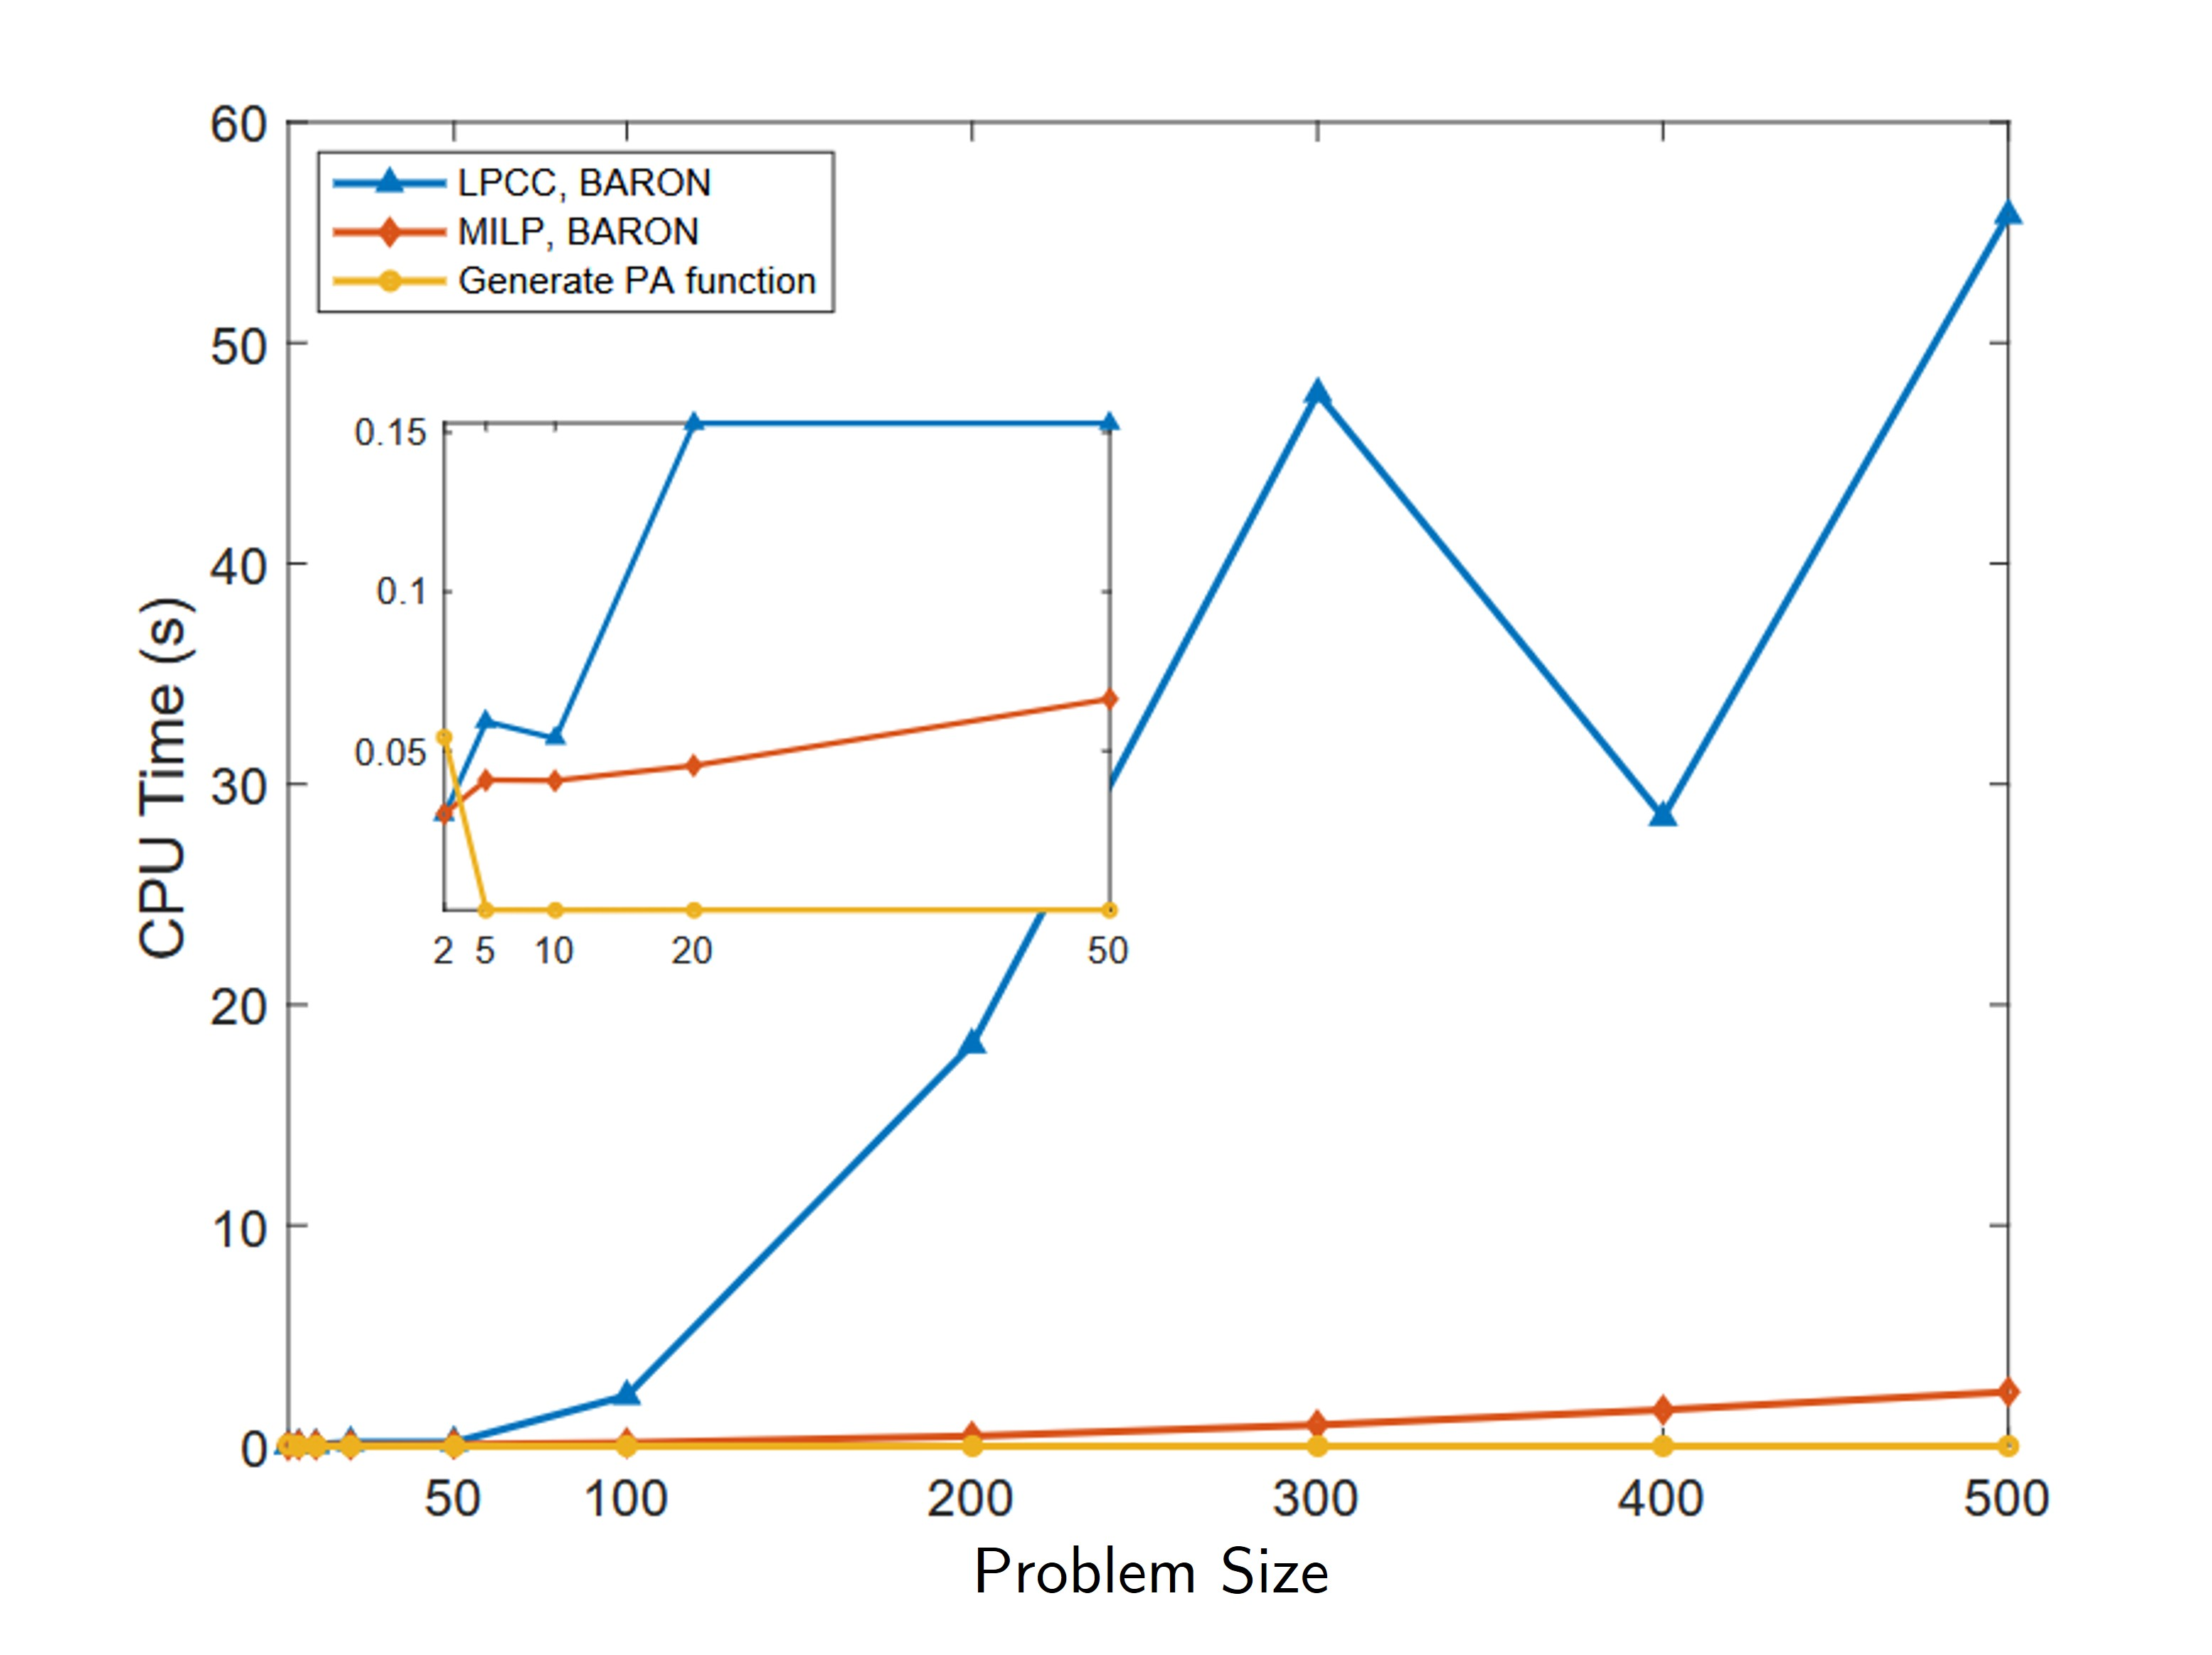
\includegraphics[width=\textwidth]{images/Root_finding_S3.jpg}
        \end{figure}
    \end{column}
\end{columns}
\end{frame}

\begin{frame}
\frametitle{Computational Complexity}
\framesubtitle{Zhang \& Khan, \emph{AD 2024}} 
	\begin{itemize}
		\item Setting up the LCP scales with polynomial complexity
		\begin{itemize}
			\item Coefficient definition includes basic algebra steps - i.e., matrix multiplication and solving linear systems 
		\end{itemize}
		\vspace{2mm}
		\item Solving LCP is computationally expensive
		\begin{itemize}
			\item Comparable to integer linear programs
			\item Preserve continuity when there's a discrete switch
		\end{itemize}
	\end{itemize}
\end{frame}

\section{New results concerning ReLU Neural Networks}
\subsection{Root finding for ReLU neural networks}
\begin{frame}{Root finding for ReLU neural networks}
\framesubtitle{(In preparation)}
\only<1>{
  	%\begin{block}{Root finding for embedded ReLU neural networks}
		\begin{itemize}
		\item \textbf{Goal}:  Given a fitted ReLU neural network $\pmb{\phi}$, solve the following for $\mathbf{x}$:
			\begin{equation*}
			\pmb{g}(\mathbf{x}, \pmb{\phi}(\mathbf{x}, p)) = 0
			\end{equation*}
		\item Where residual function $\pmb{g}: (R^n \times R^n) \rightarrow R^n$ is defined as:
			\begin{equation*}
			\pmb{g}(\mathbf{x}, \mathbf{y}) = \mathbf{P}\mathbf{x}  + \mathbf{Q}\mathbf{y} + \mathbf{r}
			\end{equation*}
		\end{itemize}
		\vspace{-2mm}
		\begin{block}{Problem Cases}
			\begin{itemize}
				\item \textbf{Case 1A}: Calculate root of neural network - i.e., solve $\pmb{\phi}(\mathbf{x}, p) = 0$. \\
				\textit{Set $\mathbf{P = 0}$, $\mathbf{Q = I}$, and $\mathbf{r = 0}$.}
				\vspace{2mm}
				\item \textbf{Case 1B}: Inverse problem of neural network - i.e., solve $\pmb{\phi}(\mathbf{x}, p) = \mathbf{r}$. \\
				\textit{Set $\mathbf{P = 0}$, $\mathbf{Q = I}$, and user-select $\mathbf{r}$.}
				\vspace{2mm}
				\item \textbf{Case 2}: Solve 1st-order neural ODE using Implicit Euler equation. \\
				 \textit{Set $\mathbf{P = I}$, $\mathbf{Q} =$ $\Delta$$t \,\mathbf{I}$, and $\mathbf{r = -x^{(k)}}$.}
			\end{itemize}		
		\end{block}
	%\end{block}
	%\vspace{-3mm}
}

\only<2>{
	\vspace{2mm}
	%%
		\begin{itemize}
		\item \textbf{Goal}: Given a fitted ReLU neural network $\pmb{\phi}$, solve the following for $\mathbf{x}$:
			\begin{equation*}
			\pmb{g}(\mathbf{x}, \pmb{\phi}(\mathbf{x}, p)) = 0
			\end{equation*}
		\item Where residual function $\pmb{g}: (R^n \times R^n) \rightarrow R^n$ is defined as:
			\begin{equation*}
			  \pmb{g}(\mathbf{x}, \mathbf{y}) = \mathbf{P}\mathbf{x}  + \mathbf{Q}\mathbf{y} + \mathbf{r}
			\end{equation*}		
		\end{itemize}
	%%
	\begin{block}{Summary of Approach}
		\begin{enumerate}
			\item ReLU NNs are piecewise affine composite functions
			\item Formulate abs-normal representation to solve $\pmb{g}(\mathbf{x}, \pmb{\phi}(\mathbf{x},p)) = \mathbf{0}$.
				\begin{equation*}
					  \begin{bmatrix}\mathbf{z} \\ \pmb{g}(\mathbf{x}, \pmb{\phi})\end{bmatrix} = \begin{bmatrix}\mathbf{c} \\ \mathbf{\overline{b}}\end{bmatrix} + \begin{bmatrix}\mathbf{Z} & \mathbf{L} \\ \mathbf{\overline{J}} & \mathbf{\overline{Y}} \end{bmatrix} \begin{bmatrix}\mathbf{x} \\ |\mathbf{z}|\end{bmatrix}
				\end{equation*}
			where the following matrices and vectors are defined:
			\vspace{-1.5mm}
				\begin{align*}
					  \mathbf{\overline{J}} &:= \mathbf{P} + \mathbf{Q}\mathbf{J} & \mathbf{\overline{Y}} &=: \mathbf{Q}\mathbf{Y} & \mathbf{\overline{b}} &=: \mathbf{r} + \mathbf{Q}\mathbf{b}
				\end{align*}
			\vspace{-7mm}
			\item Solve for $\mathbf{x}$ using complementarity approach.
		\end{enumerate}
	\end{block}
}

\only<3>{
	\vspace{1mm}
	\begin{block}{Transformations of NN to abs-normal form}
	\vspace{-1mm}
	\begin{figure}
	        \centering
	        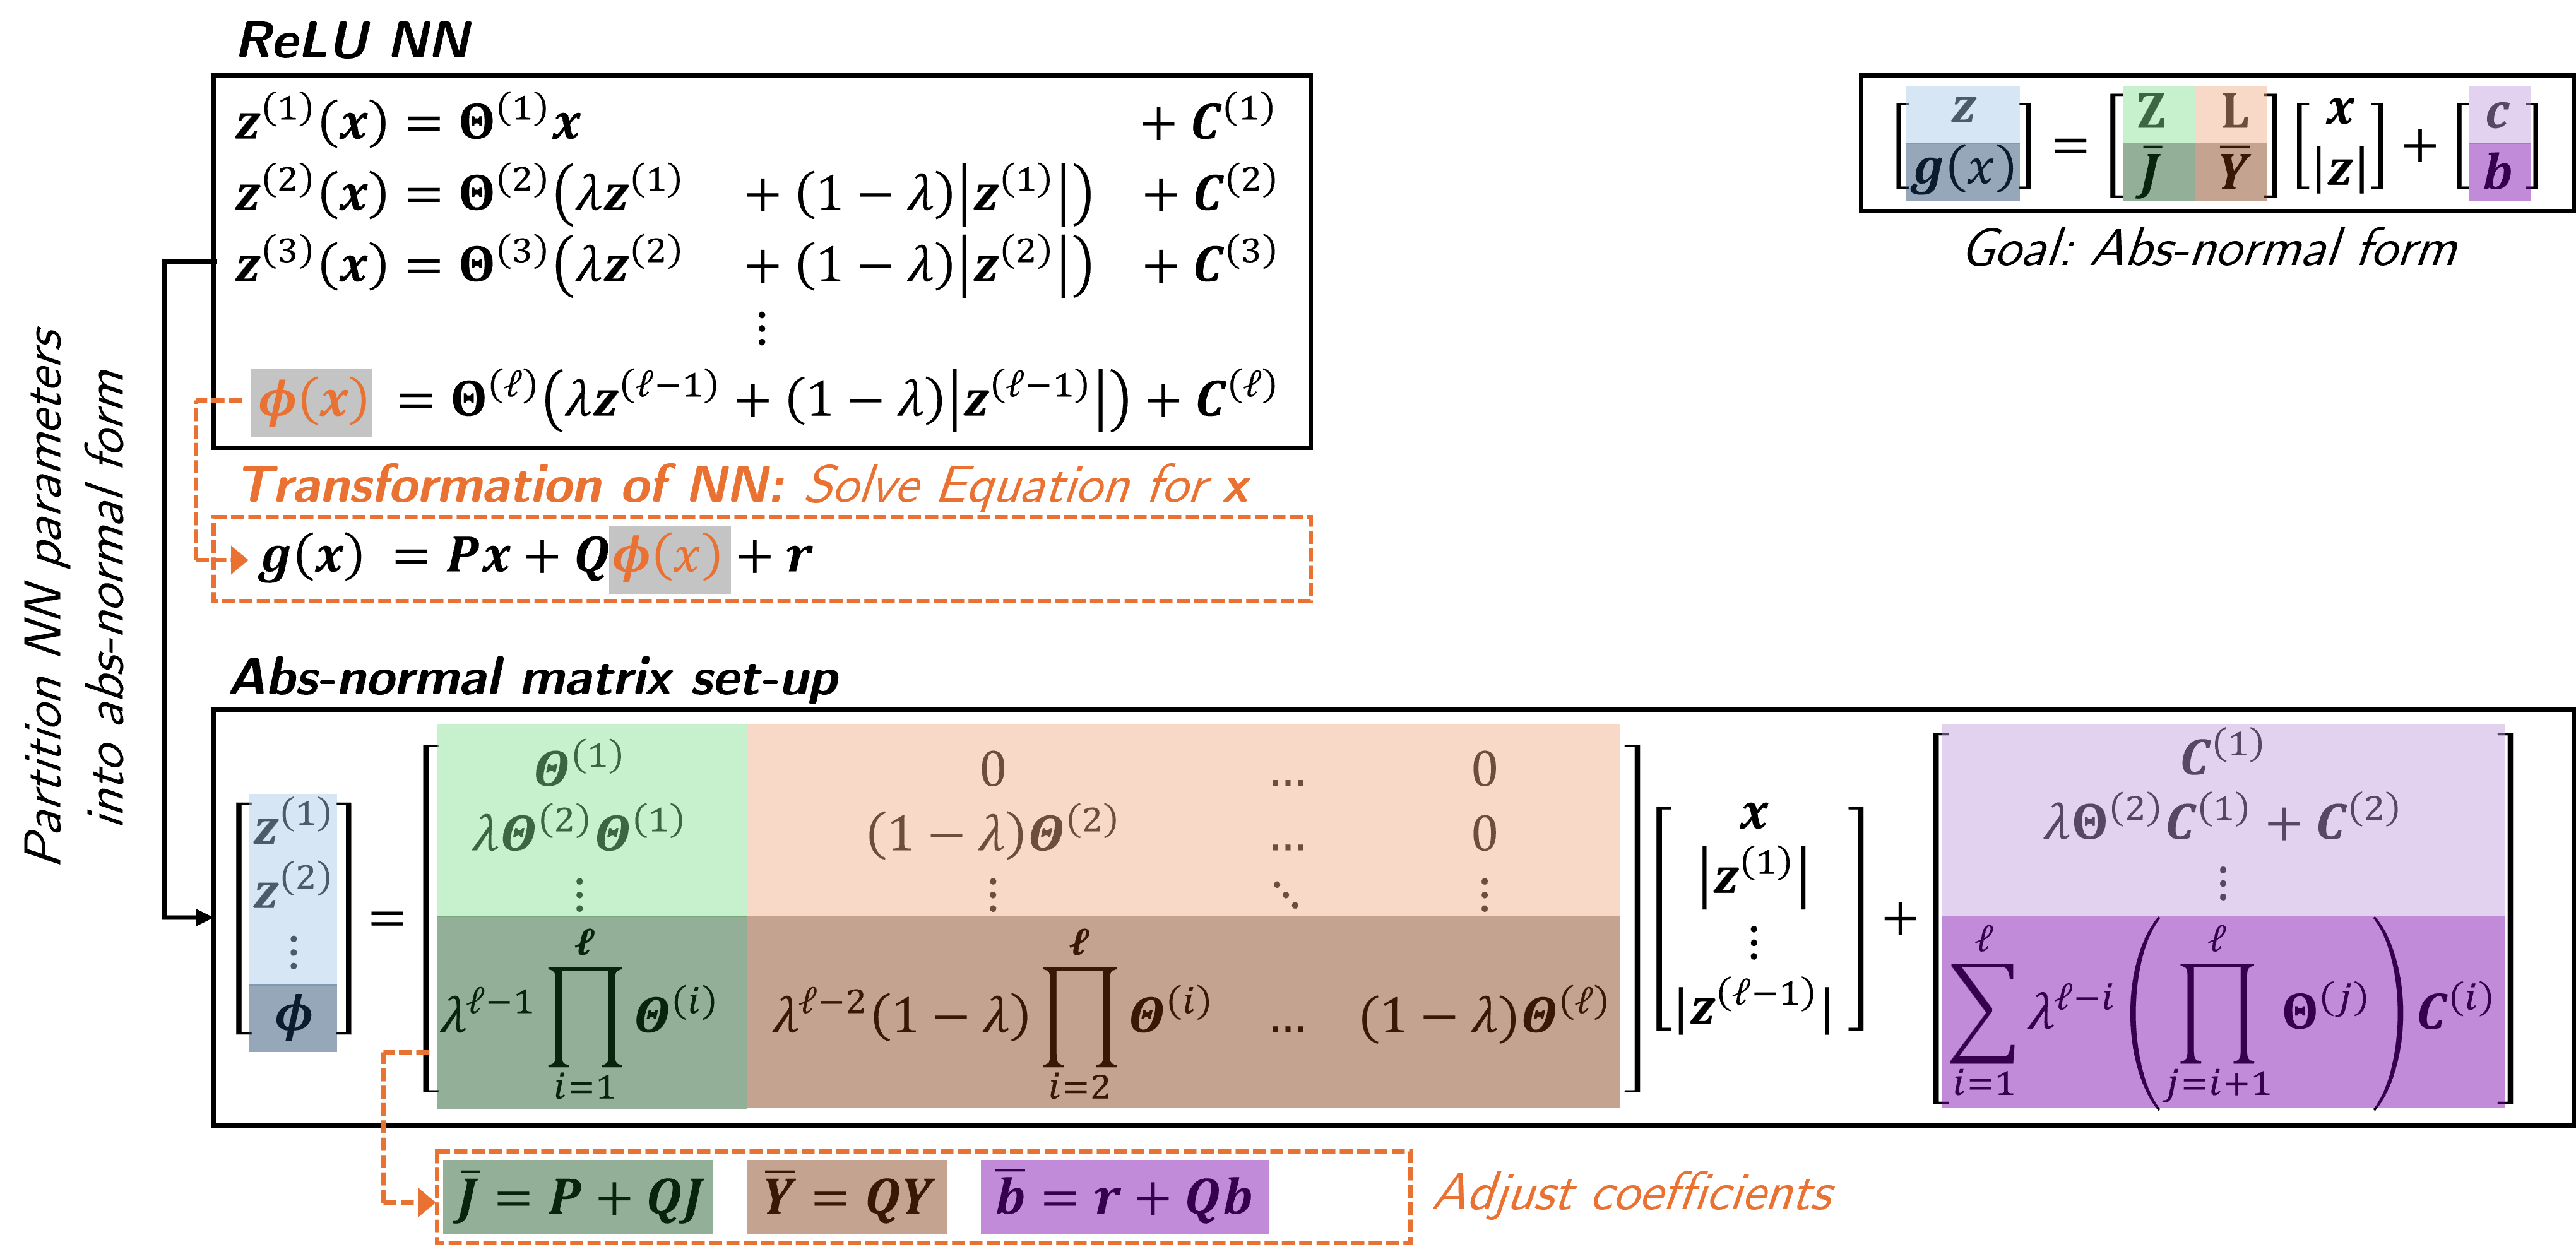
\includegraphics[width=1.0\textwidth]{images/Mapping_Transformation.png}
    	\end{figure}
	\end{block}
}

\end{frame}

\subsection{Root finding for neural ODE}
\begin{frame}{Solving neural ODEs}
\framesubtitle{(In preparation)}
\only<1>{%
	\begin{block}{Linear multistep methods to solve first order neural ODEs}
		\begin{itemize}
			\item Linear multistep methods solves root finding problems at each time step.
			\begin{itemize}
				\item \textbf{Backward Differentiation}:  
					$
					BDF_s: \,\, \sum_{k=0}^{s} a_{k} x_{n+k} - h \beta_s f(t_{n+s}, x_{n+s}) = 0, 
							\,\, \text{  where  } x' = f(t,x)
					$
				\item \textbf{Adams-Moulton}: 
					$
					AM_s: \,\, x_{s+1} - x_{s} - h \sum_{k=0}^{s} \beta_k f(t_{n+1-k}, x_{n+1-k}) = 0, 
							\,\, \text{  where  } x' = f(t,x)
					$
			\end{itemize}
			\item Coefficients for $s$-steps of multistep methods:
		\end{itemize}

	\begin{table}[ht]
	    \centering
	    \begin{tabular}{ccccc}
	        \toprule
	        Method & Order & \textbf{P} & \textbf{Q} & \textbf{r} \\
	        \midrule
	        BDF 	& 1 & $\mathbf{I}$ & $h \mathbf{I}$ 	& $-x^{(0)}$ \\
	               	& 2 & $\mathbf{I}$ & $\tfrac{2}{3}h$ 	& $-\tfrac{4}{3} x^{(1)} + \tfrac{1}{3} x^{(0)} $\\
				& ... & & & \\
	        		& s & $\mathbf{I}$ & $-\tfrac{1}{a_{s}}h\mathbf{I}$ 	& $\sum_{k=0}^{s-1} -a_k x^{(n+k)}$ \\
		   \midrule 

		   AM	& 1 & $\mathbf{I}$ & $h \mathbf{I}$ 	 & $-x^{(0)}$ \\
				& 2 & $\mathbf{I}$ & $ -\tfrac{1}{2}h\mathbf{I}$ 	& $-x^{(1)}-\tfrac{1}{2}h f(t^{(1)}, x^{(1)})$ \\
				& ... & & & \\
				& s & $\mathbf{I}$ & $-\tfrac{1}{a_{s}}h\mathbf{I}$ & $-x_{n+s-1} - h \sum_{k=1}^{s-1} \beta_{k} f(t_{n+k}, x_{n+k})$ \\
	        \bottomrule
	    \end{tabular}
	\end{table}

	\end{block}
}
\end{frame}

\begin{frame}{Implementation and Examples}
\framesubtitle{(In preparation)}
\only<1>{%
	  \begin{itemize}
	      \item Implemented in Julia v1.10.5
	      \begin{itemize}
	          \item MLCP and LCP solvers: PATHSolver.jl 1.7.5 in JuMP
	          \item Input: four matrices and two vectors of the abs-normal form
	      \end{itemize}
	  \end{itemize}
	\begin{block}{Case 1: Root of a Neural Net}
		\begin{itemize}
			\item To calculate the root of the neural net - i.e., solve $h(x, \phi) = 0$.
			\item Set $\mathbf{P = 0}$, $\mathbf{Q = I}$, and $\mathbf{r = 0}$. 
			\item Consider $\mathbf{f}(\mathbf{X}) = (\mathbf{AX}^T - \mathbf{b})^T$ where:
				\begin{equation*}
					\mathbf{A} = \begin{bmatrix} 
						\phantom{-}2 & -3 & \phantom{-}1\\
					      -4 & \phantom{-}1 & -2\\
					      \phantom{-}5 & -3 & \phantom{-}9
					\end{bmatrix},
					\mathbf{b} = \begin{bmatrix}
						\phantom{-}1 \\ \phantom{-}4 \\ -2
					\end{bmatrix}
				\end{equation*}
				A 1-layer NN mapping of $\mathbf{f}(\mathbf{X})$ produces a local solution of the root.
				\begin{equation*}
					\mathbf{x} = \begin{bmatrix} -0.276 & -0.244 & -0.019 \end{bmatrix}^T 
				\end{equation*}	
		\end{itemize}
	\end{block}
}

\only<2>{%
	\vspace{1mm}
	\begin{block}{Case 2: Trajectory of neural ODEs}
		%\begin{minipage}{0.5\textwidth}
			\begin{itemize}
				\item Consider the following CSTR ODE whose dynamics are represented using a neural network 
				where $C(0) = \begin{bmatrix} 0.09 & 0.09 & 0.00 \end{bmatrix}^T, t \in [0, 1]$.
				\vspace{-2mm}
					\begin{equation*}
						\begin{bmatrix} \dot{C_1} \\ \dot{C_2} \\ \dot{C_3} \end{bmatrix}
						 =  \begin{bmatrix}
					      -C_1 - k_1 + (C_2 + k_2)\, \text{exp} \left( \frac{k_3C_1}{C_1+2} \right) \\
					      -C_2 - k_2 - (C_2 + k_2)\, \text{exp} \left( \frac{k_3C_1}{C_1+2} \right) \\ 
					      C_1^2 + C_2^2 + k_4
					    \end{bmatrix}
					\end{equation*}
				\item \textit{Solving the BDF ($s=5$) root-finding problem at each time step produces:}
			\end{itemize}
		%\end{minipage}
		%\begin{minipage}{0.4\textwidth}
			\centering
        		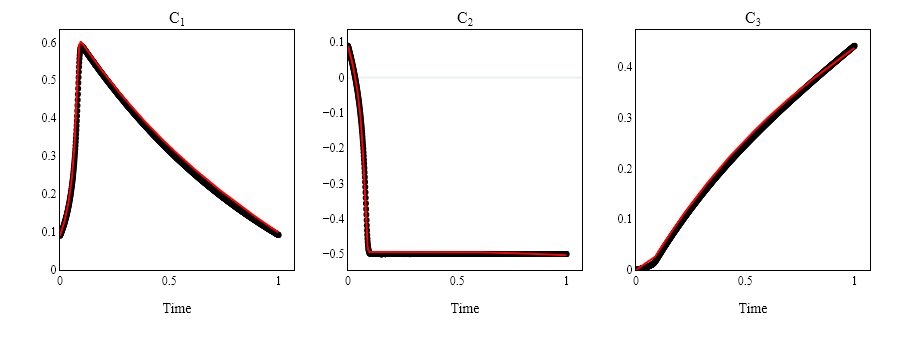
\includegraphics[width=0.65\textwidth]{images/NeuralODESolution_BFD.png}
		%\end{minipage}
	\end{block}
}

\only<3>{%
\begin{columns}[t] % Aligns content at the top
    \begin{column}{0.45\textwidth}
        \begin{itemize}\setlength{\itemsep}{10pt}
		\item The Kuramoto model describes large sets of coupled phase oscillators that synchronize with each other when interacting. 
		\item Represented as a continuous-time ODE where $\omega_i$ is unit $i$'s natural frequency and $K$ is the coupling strength.
			\begin{align*}
				\dot{\bm{\theta}_i} = \bm{\omega}_i - K \bm{r}(t) \sin(\bm{\theta}_j - \bm{\theta}_i) \\
				\bm{r}(t)e^{i\bm{\psi}(t)} = \frac{1}{N} \sum_j^N e^{i \bm{\theta}_j (t)}
			\end{align*}
		\item Consider a model with $N = 50$ oscillators and a timestep of $6\cdot 10^{-4}$. %whose dynamics are represented by a 3 layer neural network.
        \end{itemize}
    \end{column}
    
    \begin{column}{0.55\textwidth}
    \begin{itemize}
        \item Solving the root-finding problem at each time step using Euler produces:
        \vspace{1mm}
    \end{itemize}
    \vspace{-2mm}
        \begin{figure}
            \centering
            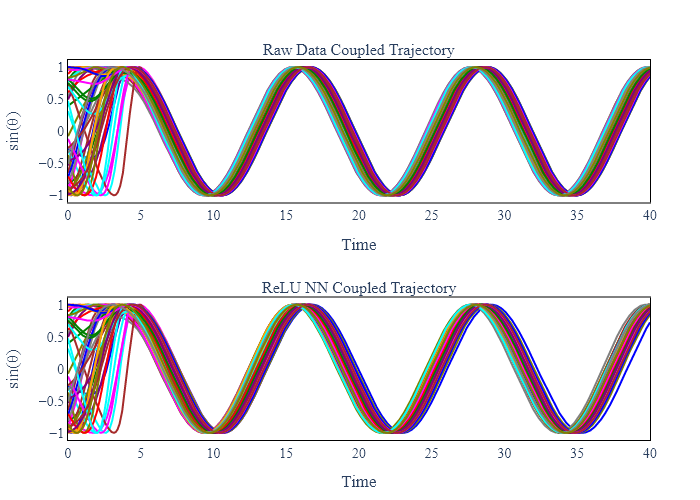
\includegraphics[width=\textwidth]{images/NeuralODE_Kuramoto.png}
        \end{figure}
    \end{column}
\end{columns}
}
\end{frame}


\section*{Conclusions}
\begin{frame}
  \frametitle{Conclusions}
  \begin{itemize}\setlength{\itemsep}{10pt}
    \item Piecewise-affine approximations for nonsmooth functions are useful and can be constructed using a forward-AD like procedure
    \item A piecewise-affine function can be represented in abs-normal form, which can be constructed using a forward-AD like procedure
    \item New root-finding approach for piecewise-affine functions, with fewer variables and equations\\
    \item New optimization formulations for piecewise-affine functions\\
    \item Verification of a global minimum can be performed before minimization\\
    \item New root-finding approaches for functions with embedded ReLU neural networks
    \item Proof-of-concept implementations developed in Julia
  \item Code available on GitHub: \\{\url{https://github.com/kamilkhanlab/abs-normal}}
  \item Funding: MACC, NSERC, ORF-RE
  \end{itemize}
\end{frame}



\end{document}
%%% Local Variables:
%%% mode: latex
%%% TeX-master: t
%%% End:
